\chapter{The magnetic structure and palaeomagnetic recording fidelity of sub-micron greigite (Fe$_3$S$_4$)}
\label{ch:res-1}

\section*{Abstract}
We present the results of a finite-element micromagnetic model of 30$\nm$ to 300$\nm$ greigite (Fe$_3$S$_4$) grains with a variety of equant morphologies. This grain size range covers the magnetic single-domain (SD) to pseudo single-domain (PSD) transition, and possibly also the PSD to multi-domain (MD) transition. The SD--PSD threshold $d_0$ is determined to be 50$\nm$ $\leq d_0 \leq$ 56$\nm$ depending on grain shape. The nudged elastic-band method was used to determine the room temperature energy barriers between stable states and thus the blocking volumes. It is found that, in the absence of interparticle magnetostatic interactions, the magnetisation of equant SD greigite is not stable on a geological scale and only PSD grains $\geq 70\,\text{nm}$ can be expected to carry a stable magnetisation over billion-year timescales, i.e., all non-interacting SD particles are essentially superparamagnetic. We further identify a mechanism for the PSD to multi-domain (MD) transition, which is of a continuous nature from PSD nucleation up to 300$\nm$, when structures typical of MD behaviour like closure domains begin to form.

\section{Introduction}
The ferrimagnetic mineral greigite (Fe$_3$S$_4$) is the iron sulphide analogue of the iron oxide magnetite (Fe$_3$O$_4$). It is commonly formed as a precursor to pyrite in early diagenetic anoxic sulphate-reducing sediments \citep{Berner1984, Hunger2007} and as a product of biomineralisation by magnetotactic bacteria \citep{Mann1990}. Although thought to be thermodynamically unstable under most sedimentary regimes, it has been found to be stable on geological timescales \citep{Roberts2011}, making greigite a possible natural remanent magnetisation (NRM) carrier in many systems, e.g., lacustrine \citep{Babinszki2007, Ron2007} and marine \citep{Roberts1993, Roberts2005, Rowan2006, Rowan2009} sediments, oil fields' shallow overburdens \citep{Abubakar2015, Donovan1984, Reynolds1993} and gas-hydrate-bearing sediments \citep{Larrasoana2007}. To further our understanding of the potential use of greigite as a proxy for environmental change, hydrocarbon exploration, magnetostratigraphy and in general the contribution of this iron sulphide to the magnetic properties of rocks, we have implemented micromagnetic numerical finite-element method (FEM) simulations of greigite. To characterise its basic properties we have modelled its magnetic domain state's shape and size dependence using the \textit{DUNLOP} package \citep{Nagy2016} and its stability on geological timescales at room temperature using the \textit{MERRILL} package \citep{Nagy2017}.\par

The model solutions are dependent on a balance between various magnetic forces and thus it is important that the material's magnetic parameters be known as accurately as possible. Past difficulties in producing pure greigite samples on which to determine these parameters has resulted in a lack of accurate models in the literature. However, these difficulties have been overcome, and recent measurements on highly pure, high crystallinity synthetic greigite samples \citep{Chang2008,Chang2009,Li2014,Winklhofer2014} now allow for numerical micromagnetic models to probe the magnetic microstructure of greigite.\par

The fundamental magnetic parameters of greigite used in this investigation are the saturation magnetisation $M_\text{S}=3.51\,\mu_\text{B}\,\text{p.c.u.}$ \citep{Li2014} or $\roughly 2.7 \times 10^5\,\text{A/m}$  which is $\roughly$11\% higher than the value reported by \citet{Chang2009} of $3.25\,\mu_\text{B}$ p.c.u. (and $\roughly$57\% the value of  $M_\text{S}$ for magnetite) and the exchange stiffness constant $A=2\times10^{-12}\,\text{J}/\text{m}$ \citep{Chang2008} ($\roughly$15\% the value of $A$ for magnetite). \citet{Winklhofer2014} estimated a cubic magnetocrystalline anisotropy (MCA) term $K_1=-1.7\times10^4\,\text{J}/\text{m}^3$ ($\roughly$42\% higher than the value for magnetite) and negligible second MCA constant $K_2$ to $K_1$ ratio, i.e., the easy axes are the $<$111$>$.\par

Very few micromagnetic models of greigite have so far been attempted, with only the work of \citet{Muxworthy2013} having been published. They implemented a micromagnetic finite-difference (FD) method that used the earlier value of $M_\text{S}$ from \citet{Chang2009} to model both individual grains and the effects of magnetostatic interactions between cuboidal particles of greigite arranged in chains. For the single crystals they found good agreement with the analytical calculations of \citet{Diaz-Ricci1992} (for which crude estimates of the magnetic parameters were used). However, due to their structured spatial discretisation, FD methods are not as well suited for the simulation of the euhedral morphologies seen in natural samples \citep{Snowball1997} as FEMs are. Elongation is a common feature of magnetosomal grains but not of particles with non-biogenic origin. Although \citet{Muxworthy2013} have demonstrated that particle elongation and interparticle magnetostatic interactions are important, this study is limited to a variety of equant, isolated particles whose behaviour represent the limit as the particle concentration approaches zero. As such, this study provides a first step towards a more complete picture of the role of non-biogenic greigite in rock magnetics.\par

The grain size of a magnetic mineral strongly affects its magnetic behaviour and palaeomagnetic recording fidelity. As grain size distributions are usually inferred from bulk magnetic properties, a deep understanding of how a grain's magnetic properties depend on size is needed. We present here the results of a numerical FEM study of the stress-free, zero-field domain states of spherical and equant euhedral single grains of greigite in the single-domain (SD) to pseudo single-domain (PSD) range. To address this question we used the nudged elastic-band (NEB) method \citep{Fabian2017} to calculate action-minimising paths (AMPs) between stable magnetic configurations which allow us to determine energy barriers and from these the blocking volumes of naturally occurring equant euhedral grains of greigite.\par
%-----------------------------------------------------

\section{Methodology}
\subsection{The micromagnetic algorithm}
For a ferromagnetic (in the broad sense, i.e., ferro- or ferri-) material{\textemdash}neglecting external fields, thermal and magnetostrictive effects{\textemdash}the Gibbs free-energy functional can be written as \citep{Brown}
\begin{equation}
E_\text{G} = \int_{\Omega} (\phi_{\text{exchange}} + \phi_{\text{anisotropy}} + \phi_{\text{stray}})\,\text{d}^3 \boldsymbol{r},
\end{equation}
with $\Omega$ the ferromagnetic volume. Here,
\begin{equation}
\phi_{\text{exchange}}=A|\nabla\boldsymbol{m}|^2,
\end{equation}
 with the reduced (unitary) magnetisation vector $\boldsymbol{m}$, is the expression for the continuum approximation of the energy density due to the quantum-mechanical exchange forces \citep{Landau1935}.\par

\begin{equation}
\phi_{\text{anisotropy}}=\frac{K_1}{2}\sum_{i\neq j}\gamma_i^2\gamma_j^2 + K_2\prod_i\gamma_i^2,
\end{equation}
with $\gamma_i$ the direction cosines, is the MCA energy density in the cubic anisotropy system. In the cartesian system this has the form:
\begin{equation}
\phi_{\text{anisotropy}}=K_1(m_x^2m_y^2+m_y^2m_z^2+m_z^2m_x^2),
\end{equation}
where $K_2$ has been neglected since in the cubic anisotropy system we are assuming, $K_1$ is the dominant term at room temperature. Finally,
\begin{equation}
\phi_{\text{stray}}=-\frac{\mu_0M_\text{S}}{2}\boldsymbol{m}\cdot\boldsymbol{H}_{\text{stray}}
\end{equation}
is the magnetostatic self-energy density, with $\boldsymbol{H}_{\text{stray}}$ the stray field produced by the ferromagnetic body. It is known from thermodynamics that under isothermal and isobaric conditions a system will spontaneously evolve towards an equilibrium state with minimal Gibbs free-energy. It is the aim of a micromagnetic algorithm to find the equilibrium magnetisation $\boldsymbol{m}$.\par

The variational principle proposed by \citet{Brown} $\delta E_\text{G} / \delta \boldsymbol{m}=0$ leads to `Brown's equations'
\begin{equation}
\boldsymbol{m}\times \left( \boldsymbol{H}_\text{exchange} + \boldsymbol{H}_\text{anisotropy} + \boldsymbol{H}_\text{stray}\right) = 0,
\end{equation}
with
\begin{equation}
\boldsymbol{H}_\text{exchange} = \frac{2A}{\mu_0M_\text{S}} \nabla^2\boldsymbol{m}
\end{equation}
and
\begin{equation}
\boldsymbol{H}_\text{anisotropy} = \frac{2K_1}{\mu_0M_\text{S}}[m_x(1-m_x^2)\ihat + m_y(1-m_y^2)\jhat + m_z(1-m_z^2)\boldsymbol{\hat{k}}].
\end{equation}
Therefore, in equilibrium the magnetisation is parallel to an \emph{effective} field $\boldsymbol{H}_\text{eff.} = \boldsymbol{H}_\text{exchange} + \boldsymbol{H}_\text{anis} + \boldsymbol{H}_\text{stray}$, while $\mu_0M_\text{S}\boldsymbol{m}\times\boldsymbol{H}_\text{eff.}$ is the local torque produced on the magnetisation by the effective field at each magnetic site, so we have equilibrium via the vanishing of the torque \citep{Brown}.\par

We thus have the two main approaches towards finding a micromagnetic solution, i.e., the minimisation of the Gibbs free-energy functional, which is faster though prone to false minima, and the vanishing of the torque, which is slower but more robust and physically meaningful \citep{Gilbert2004}. The former is usually achieved with a variety of gradient descent methods \citep{Fischbacher2017} while the latter by numerical integration of the Landau-Lifshitz-Gilbert (LLG) equation \citep{Gilbert2004}
\begin{equation}\label{llg}
\frac{\partial \boldsymbol{m}}{\partial t} = -\gamma^{'} \boldsymbol{m}\times\boldsymbol{H}_{\text{eff}} - \alpha\gamma^{'}\boldsymbol{m}\times(\boldsymbol{m}\times\boldsymbol{H}_{\text{eff}}) \, ,
\end{equation}
where $\alpha$ is a phenomenological damping constant, and $\gamma^{'} = \gamma /(1+\alpha^2)$ with $\gamma$ the gyromagnetic ratio.\par

FEMs allow for an unstructured discretisation of the spatial domain which in our case is decomposed into tetrahedral elements. In the treatment of the micromagnetic theory of \citet{Brown} there are some linearisations, which means that there should not be large variations in the direction of $\boldsymbol{m}$ between neigbouring nodes in the FE mesh. To model nonuniform structures it is sufficient that the spatial discretisation in the model be smaller than the exchange length $l_\text{exch.} = \sqrt{2A/\mu_0M_\text{S}^2}$ \citep{Rave1998}, which for greigite is $l_\text{exch.} \approx 6.6\, \text{nm}$; a maximum element size of 5$\nm$ has been chosen for all the models. The non-local problem of calculating the stray field is handled via a transformation method \citep{Imhoff1990} in \textit{DUNLOP} and by a hybrid finite-element/boundary-element formulation \citep{Fredkin1990} in \textit{MERRILL}.\par

\subsection{Choice of morphologies}
Based on scanning electron microscopy (SEM) and transmission electron microscopy (TEM) micrographs of synthetic greigite samples \citep{Chang2008, Li2014} and of naturally occuring samples \citep{Snowball1997, Vasiliev2008}, five octahedral shapes have been chosen with increasing degrees of truncation of their corners: from no truncation at all (octahedron) to a `completely' truncated shape (cuboctahedron) and three truncated octahedral shapes in-between to which we further refer to as minimally truncated octahedron, truncated octahedron (the regular case), and maximally truncated octahedron (Fig. \ref{fig1}). This series of shapes models the influence of the ratio of $\{001\}$ to $\{111\}$ faces, which increases with truncation. Furthermore, spherical shapes which, although unrealistic, serve as `control subjects' that do not exhibit configurational anisotropy \citep{Williams2006} and cubic shapes which have been modelled before by \citet{Muxworthy2013} and represent the case of only $\{001\}$ faces. All the volumes are normalised to cubes, i.e., a particle sized 120$\nm$ has a volume of (120$\nm$)$^3$.
\begin{figure}
\centering
%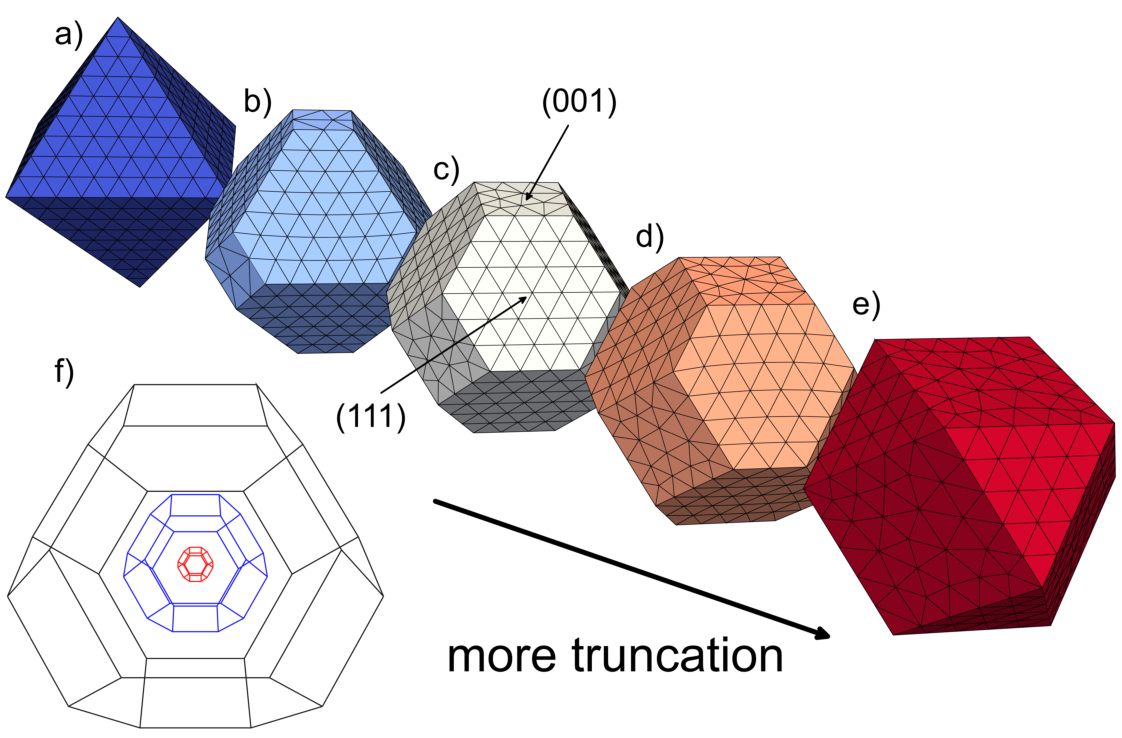
\includegraphics[width=\textwidth]{Figure_01_HR.pdf}
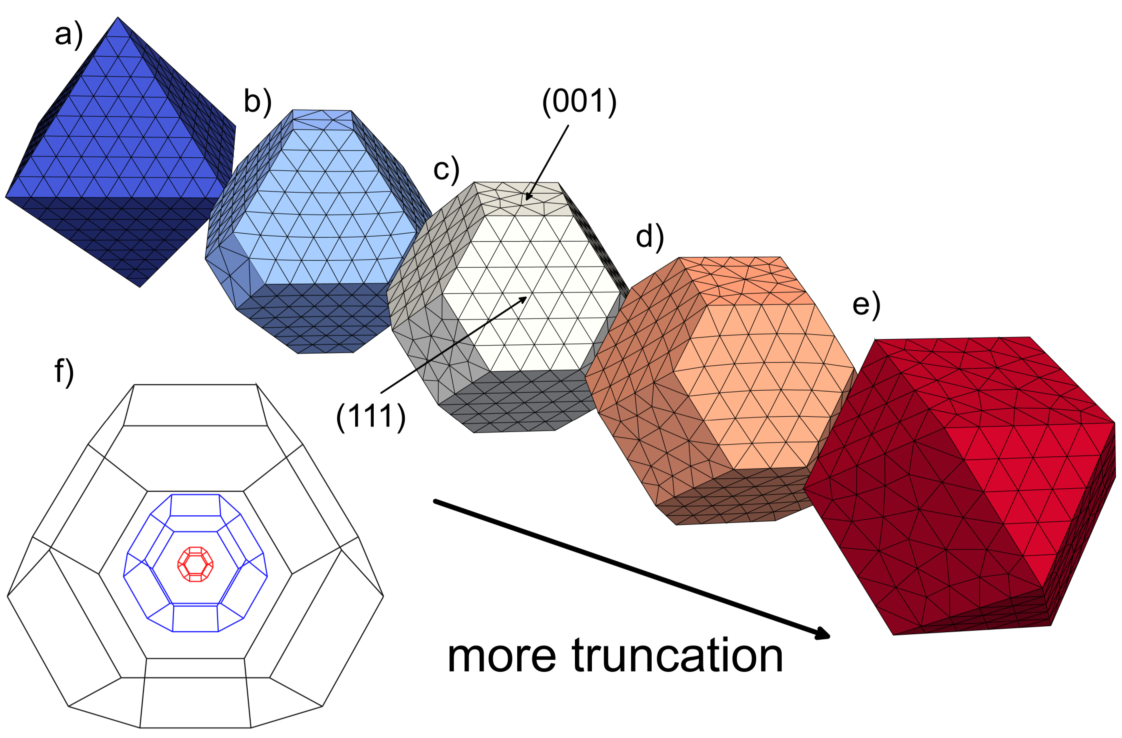
\includegraphics[width=\textwidth]{research-1/figs/Figure_01.pdf}
\caption[FE meshes of the model euhedral geometries]{FE meshes of the model euhedral geometries. From a) a regular octahedron, the rest are obtained by increasingly cutting more off the corners such that the edges of the octahedron are: b) halved (min. t. octahedron); c) reduced to a third (regular t. octahedron); d) reduced to a quarter (max. t. octahedron). e) A regular cuboctahedron is obtained by truncating to the point where the octahedron edges disappear entirely. The easy axes of magnetisation are the $<$111$>$ and the hard are the $<$001$>$, which are normal to the hexagonal $\{111\}$ and square $\{001\}$ faces, respectively, of the truncated octahedra. For a sense of scale, f) three nested regular truncated octahedra are shown with sizes 30$\nm$ (red), 120$\nm$ (blue) and 300$\nm$ (black).}
\label{fig1}
\end{figure}

\subsection{Crystal growth model}
The magnetic domain structure of a ferromagnetic nanoparticle obtained by a micromagnetic algorithm is not only a function of its mineralogy, size and shape, but also of its history. In particular, it is known that a SD particle can grow and remain SD up to a threshold size $\dmax$ after which it will become PSD \citep{Enkin1994}. (In this study we are concerned with the zero-field microstructure and properties; in this context, the onset of PSD beheaviour is marked by the formation of a single-vortex structure). If the particle then decreases its volume it will remain PSD down to a threshold $\dmin$ ($< \dmax$) below which it will become SD again. This defines a size range in which a ferromagnetic grain can be either SD or PSD dependent on its history \citep{Muxworthy2006}. This phenomenon has been modelled for the seven morphologies (Fig. \ref{fig1}) in the 30$\nm$ to 300$\nm$ size range.\par

Starting from a 30$\nm$ particle, we obtain the micromagnetic solution and extrapolate it to a larger grain. This becomes the new initial condition for which we solve and repeat, growing the particle in steps of 2$\nm$. Since a very fine incremental size step is used, much smaller than the exchange length, we can be certain that we are not missing any features from one step to the next. This process accurately models grain growth.\par

Once the particles have grown to 120$\nm$, the procedure is then reversed in decreasing steps of 2$\nm$ until the initial size of 30$\nm$ is reached. Since chemical alteration usually proceeds by alteration of the surfaces, the volume decreasing process can be thought of as a model for chemical alteration to a non-magnetic phase. This growth from 30$\nm$ to 120$\nm$ followed by the reverse process is referred to as the \textit{main loop} (ML).\par

Solutions on the size-descending curve not found on the size-increasing curve were also subject to growth; the \textit{secondary loop} (SL). The ML and SL allow us to investigate the different domain states with size, shape and history. These micromagnetic solutions were performed by numerical integration of the LLG equation (Eqn. \ref{llg}). Stable solutions at 120$\nm$, whether found on the ML or SL, were further grown up to 300$\nm$. Energy minimisation was used for calculations larger than 120$\,$nm, as integration of the LLG equation is prohibitively slow at these sizes. The parallel \textit{DUNLOP} package \citep{Nagy2016} was used to model these grain size dependencies.\par

These models overlook the effect of thermal fluctuations. However, this limitation is addressed by calculation of the relaxation times. These allow the determination of the particles domain state at a given size beyond the capabilities of standard micromagnetics.\par

\subsection{Relaxation times}
Over a sufficiently long observation time, termed the \textit{relaxation time}, a ferromagnetic particle will switch between different stable states due to thermal activation. The relaxation time is given by \citep{Neel1955}
\begin{equation}\label{neel}
\tau = \tau_0 \exp\left(E_{B}/K_{\text{B}}T\right),
\end{equation}
where $K_{\text{B}}$ is Boltzmann's constant, $T$ the temperature at which the transition occurs and $\tau_0$ the \textit{attempt time}, commonly with a value of $\roughly$10$^{-9}\,$s \citep{McNab1968}. Any transition between stable states must occur along an AMP \citep{Fabian2017}; $E_B$ is the energy barrier along such a path. When $E_B$ is of the order of the thermal energy available on a timescale of interest, a particle is in a superparamagnetic (SP) state, spontaneously switching back and forth between different SD orientations. SD grains with an energy barrier larger than $\roughly60\,K_\text{B}T$ have a relaxation time in the order of billions of years and are thus considered stable SD (SSD) reliable palaeomagnetic recorders \citep{Dunlop}. The SP--SSD threshold is therefore one of the key parameters to assess the palaeomagnetic significance of a NRM. A NEB method \citep{Fabian2017} has been implemented in the micromagnetic package \textit{MERRILL} \citep{Nagy2017} (such methods are currently unavailable in \textit{DUNLOP}) to calculate the energy barriers between the stable configurations for the (truncated) octahedral particles, from 30$\nm$ increasing in steps of 2$\nm$ until the blocking volume is reached, which is here taken to be the volume for which the relaxation time surpasses four billion years.\par

Unlike early NEB methods (as applied to magnetic systems) which approximated each particle as a single dipole \citep{Berkov1998}, here we are concerned with full micromagnetic solutions and thus, our results extend beyond SD configurations and coherent rotations. A similar method was implemented by \citet{Dittrich2002} to study the energy barriers in patterned granular media.\par
%-----------------------------------------------------

\section{Results and Discussion}
\subsection{Magnetic structure in the SD--PSD regime}\label{sd-psd}
Starting at 30$\nm$ from a randomised initial condition, all shapes relax to a SD state along an easy direction. Extrapolating onto larger grains, this state remains stable up to a threshold $\dmax$ (Figs. \ref{fig2}a, c). When the SD state solutions are grown beyond $\dmax$, they are found to relax to an easy aligned vortex (EAV) (Figs. \ref{fig2}a, d). For all shapes, this vortex configuration is stable up to 120$\nm$. On reversal, the EAV is stable down to a threshold $d_{\text{EH}}$ (Fig. \ref{fig2}a). Below $d_{\text{EH}}$, the EAV goes to a hard-aligned vortex (HAV) preserving its chirality (Figs. \ref{fig2}a, e). Further decreasing the volume, the HAV is stable down to $\dmin$ and below that, the HAV relaxes back to SD (Fig. \ref{fig2}a). This general behaviour on the ML is referred to as Type 1 (Figs. \ref{fig2}a, \ref{fig3}a, e, g, k), for which we introduce the notation:
\begin{equation}\label{type1}
\text{T}_1=\underbrace{\left(\text{SD}_{30}^{\dmax}\rightarrow\text{EAV}_{\dmax}^{120}\right)_{\rightarrow}}_\text{growth part} +
\underbrace{\left(\text{EAV}_{120}^{d_{\text{EH}}}\rightarrow\text{HAV}_{d_{\text{EH}}}^{\dmin}\rightarrow\text{SD}_{\dmin}^{30}\right)_{\leftarrow}}_\text{volume-decreasing part},
\end{equation}
with $30\,\text{nm}<\dmin<d_{\text{EH}}<\dmax<120\,\text{nm}$.\par
\begin{figure}
\centering
%\includegraphics[width=\textwidth]{Figure_02_HR.pdf}
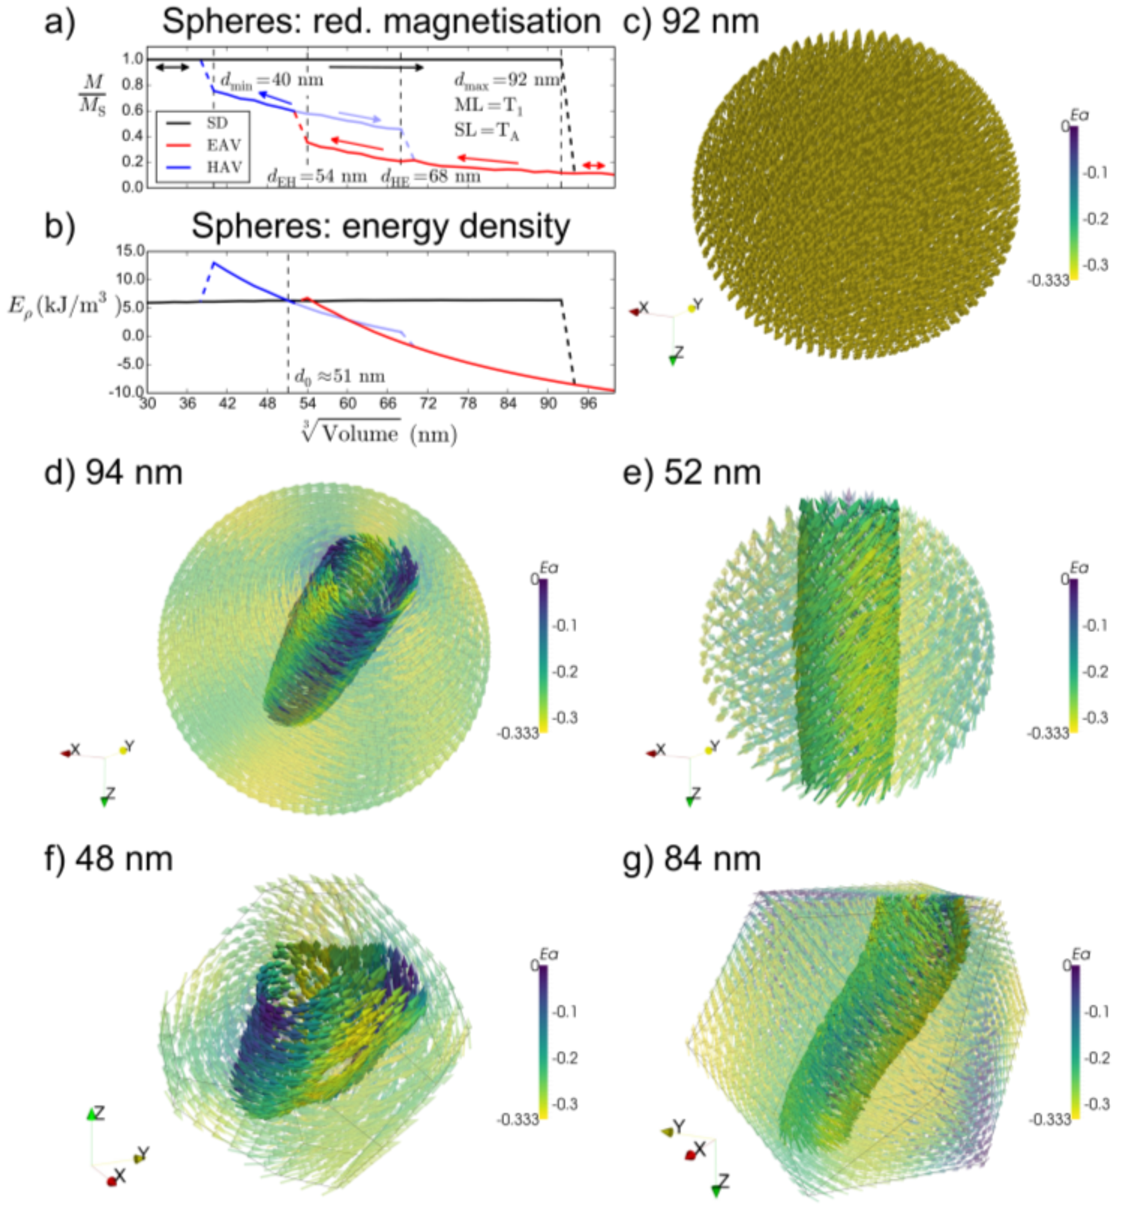
\includegraphics[width=\textwidth]{research-1/figs/Figure_02.pdf}
\caption[Micromagnetic structures of spheres and intermediate-aligned vortex states]{Micromagnetic structures of spheres and intermediate-aligned vortex states. Reduced magnetisation (a) and energy density (b) against size. The SD [$\bar{1}\bar{1}\bar{1}$] state is numerically stable up to $\dmax=92\,\text{nm}$ (c). Growing this solution to a 94$\nm$ grain it is found to relax to a [$\bar{1}\bar{1}\bar{1}$] EAV (d), stable up to 120$\nm$. The EAV is then interpolated into smaller grains, stable down to $d_\text{EH}=54\,\text{nm}$ (a). At 52$\nm$ the EAV goes to a [00$\bar{1}$] HAV (e), stable down to $\dmin=40\,\text{nm}$. At 38$\nm$, the solution relaxes to the original SD state (a). This sequence is referred to as a Type 1 \textit{main loop} (ML). Growth of the HAV from 52$\nm$ forms the Type A \textit{secondary loop} (SL): the HAV is found to be stable up to $d_{\text{HE}}=68\,\text{nm}$ (a) and to realign with the easy direction at 70$\nm$. Vortex states can not only be easy or hard-aligned, but also $<$011$>$ intermediate-aligned vortices (IAVs) (f) and distorted IAV configurations (dIAV) (g). MLs in which IAVs are found are referred to as Type 2. Colour represents the MCA energy normalised by $|K_1|$. The vortex cores are highlighted by obtaining a helicity ($K=\boldsymbol{m}\cdot\nabla\times\boldsymbol{m}$) isosurface and reducing the opacity of the rest of the arrows.}
\label{fig2}
\end{figure}

Another sequence was observed. On the size-descending curve, the EAV is stable down to a threshold $d_{\text{EI}}$ below which the EAV goes to a $<$011$>$ intermediate-aligned vortex (IAV) (Figs. \ref{fig2}f, g), stable down to $d_{\text{IH}}$. Below that, the IAV goes to a HAV which remains down to $\dmin$. Finally, below $\dmin$ the HAV relaxes back to SD. This ML behaviour is referred to as Type 2 (Figs. \ref{fig3}c, i), with the formula:
\begin{equation}\label{type2}
\text{T}_2=\underbrace{\left(\text{SD}_{30}^{\dmax}\rightarrow\text{EAV}_{\dmax}^{120}\right)_{\rightarrow}}_\text{growth part} +
\underbrace{\left(\text{EAV}_{120}^{d_{\text{EI}}}\rightarrow\text{IAV}_{d_{\text{EI}}}^{d_{\text{IH}}}\rightarrow\text{HAV}_{d_{\text{IH}}}^{\dmin}\rightarrow\text{SD}_{\dmin}^{30}\right)_{\leftarrow}}_\text{volume-decreasing part},
\end{equation}
with $30\,\text{nm}<\dmin<d_{\text{IH}}<d_{\text{EI}}<\dmax<120\,\text{nm}$.\par

Growth of the vortex configurations found on the size-descending curve (HAVs, IAVs) forms the SL. When the ML is Type 1, the HAV is grown up to a threshold $d_\text{HE}$ beyond which it realigns with an easy direction (Fig. \ref{fig2}a). When the ML is Type 2, the HAV goes to either an EAV (Fig. \ref{fig3}c) or to the IAV it nucleated from (Fig. \ref{fig3}i). When the IAV is grown beyond a threshold $d_\text{IE}$ it realigns with an easy direction (Fig. \ref{fig3}c). This behaviour on the SL is referred to as Type A (Fig. \ref{fig2}a, \ref{fig3}c, e, g), with the general formula (in the case of growth of the HAV and realignment to an EAV):
\begin{equation}\label{typeA}
\text{T}_{\text{A}}=\underbrace{\left(\text{HAV}_{d_{\text{EH}}}^{d_{\text{HE}}}\rightarrow\text{EAV}_{d_{\text{HE}}}^{120}\right)_{\rightarrow}}_\text{secondary growth part}.
\end{equation}
There is also the possibility that the HAV/IAV is stable up to 120$\nm$. This SL is a Type B (Fig. \ref{fig3}a, i, k), with the general formula (in the case of growth of the HAV):
\begin{equation}\label{typeB}
\text{T}_{\text{B}}=\underbrace{\left(\text{HAV}_{d_{\text{EH}}}^{120}\right)_{\rightarrow}}_\text{secondary growth part}.
\end{equation}
\begin{figure}
\centering
%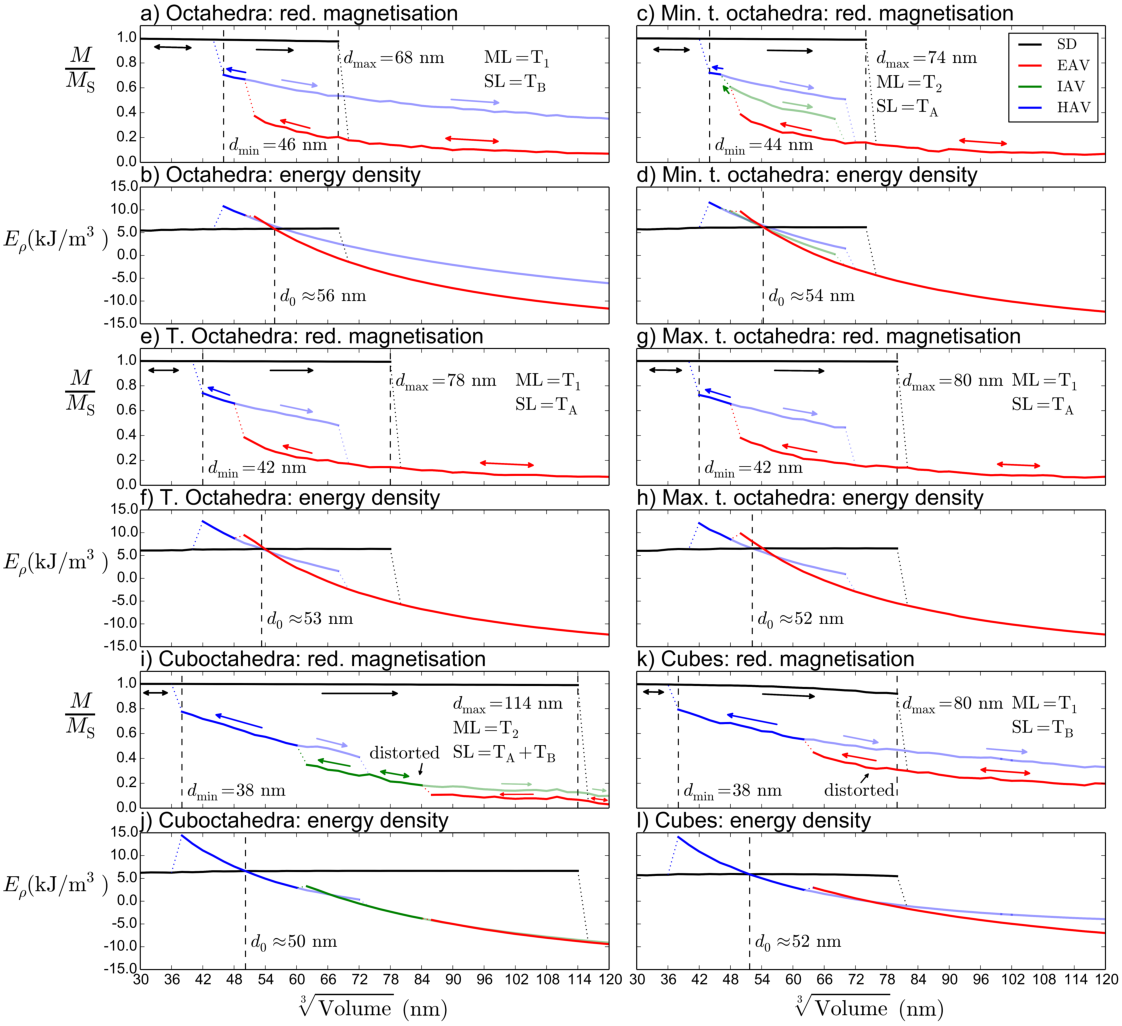
\includegraphics[width=\textwidth]{Figure_03_HR.pdf}
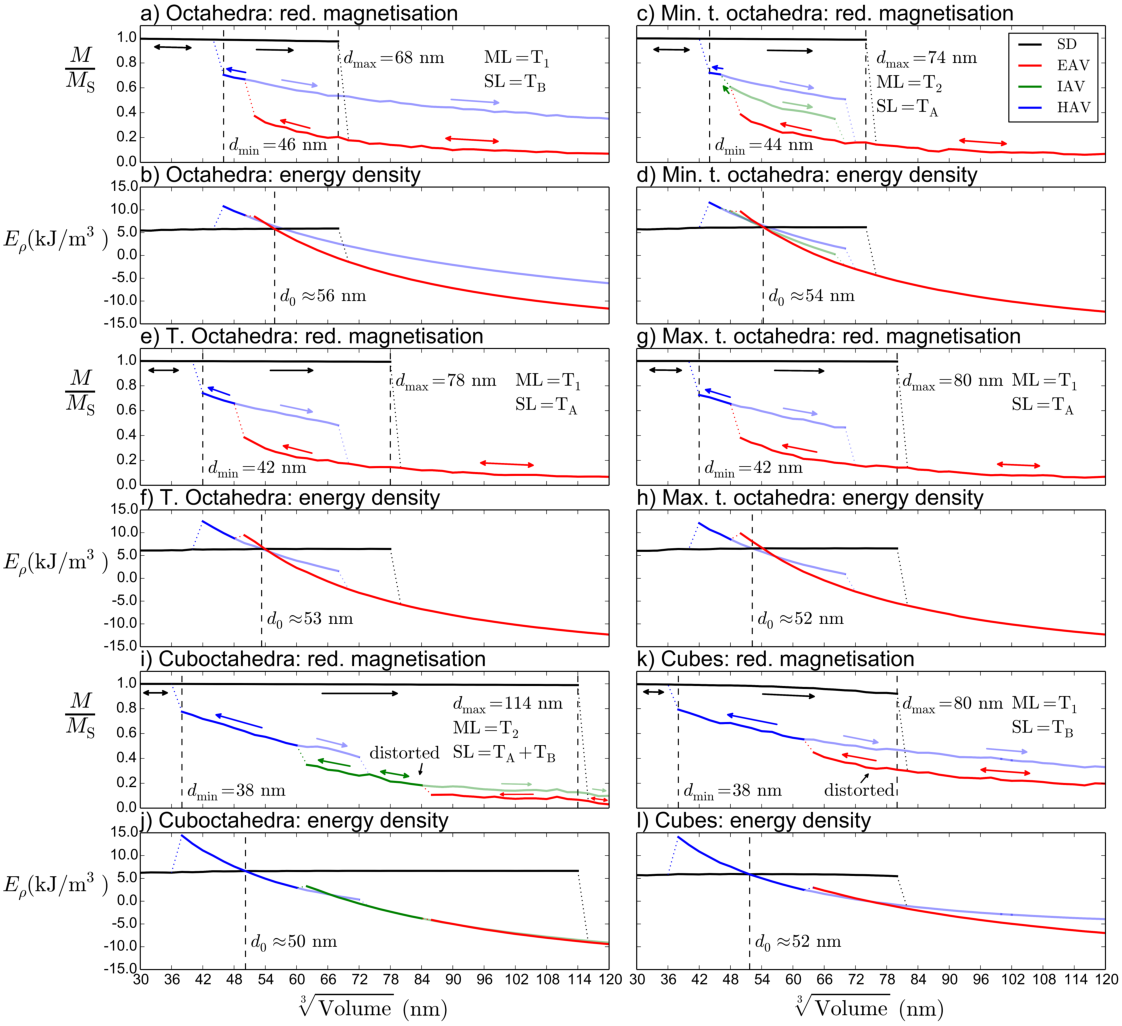
\includegraphics[width=\textwidth]{research-1/figs/Figure_03.pdf}
\caption[Domain states and energies in the SD--PSD transition regime]{Domain states and energies in the SD--PSD transition regime. Reduced magnetisation (a, c, e, g, i, k) and energy density (b, d, f, h, j, l) against size. All shapes relax to an easy aligned SD state at 30 nm from a randomised initial condition. The SD state is numerically stable up to $\dmax$ (black lines). Growth beyond $\dmax$ results in the magnetisation relaxing to an EAV, stable up to 120$\nm$ (red lines). The solution is then interpolated into smaller grains. This forms the \textit{main loop} (ML) (opaque lines). The EAV is stable down to a threshold beyond which a HAV is nucleated on the size-descending curve. The HAV is stable down to $\dmin$, below which it relaxes to a SD state. This is a Type 1 ML (a, e, g, k). When the EAV goes through an IAV (green lines) before going to the HAV configuration the ML is Type 2 (c, i). Growth of the HAVs and IAVs found on the size-descending curve forms the \textit{secondary loop} (SL) (translucent lines). When these realign with the EAV or with the vortex state they nucleated from the SL is Type A (c, e, g, i (translucent blue line)). When they are stable up to 120$\nm$ the SL is Type B (a, i (translucent green line), k).}
\label{fig3}
\end{figure}

\subsubsection{Spheres}
Fig. \ref{fig2}a shows the reduced magnetisation and Fig. \ref{fig2}b the energy density (against size) for the spherical shapes. Spheres showed a Type 1 ML (Eq. \ref{type1}), with a specific formula:
\begin{equation}
\text{ML}_{\text{sph.}}=\left(\text{SD}_{30}^{92}\rightarrow\text{EAV}_{94}^{120}\right)_{\rightarrow} + \\
\left(\text{EAV}_{120}^{54}\rightarrow\text{HAV}_{52}^{40}\rightarrow\text{SD}_{38}^{30}\right)_{\leftarrow}.
\end{equation}
The SD state at $\dmax=92\,\text{nm}$ and the EAV at 94$\nm$ are shown in Figs. \ref{fig2}c--d. The SL is formed by growing the HAV found at 52$\nm$ (Fig. \ref{fig2}e). This is a Type A SL (Eq. \ref{typeA}), with formula:
\begin{equation}
\text{SL}_{\text{sph.}}=\left(\text{HAV}_{52}^{68}\rightarrow\text{EAV}_{70}^{120}\right)_{\rightarrow}.
\end{equation}
\par

\subsubsection{Octahedra and truncated octahedra}
Fig. \ref{fig3} shows the reduced magnetisation and energy density plots for the rest of the shapes. The octahedra (Figs. \ref{fig3}a--b) showed a Type 1 ML (Eq. \ref{type1}), specifically:
\begin{equation}
\text{ML}_{\text{oct.}}=\left(\text{SD}_{30}^{68}\rightarrow\text{EAV}_{70}^{120}\right)_{\rightarrow} + \\
\left(\text{EAV}_{120}^{52}\rightarrow\text{HAV}_{50}^{46}\rightarrow\text{SD}_{44}^{30}\right)_{\leftarrow}.
\end{equation}
The SD state at $\dmax=68\,\text{nm}$ (Fig. \ref{fig4}a) shows significant flowering{\textemdash}deflection of the magnetisation onto edges and vertices. The EAV nucleated at 70$\nm$ is shown in Fig. \ref{fig4}b. Growth of the HAV nucleated at 50$\nm$ (Fig. \ref{fig4}c) showed a Type B SL (Eq. \ref{typeB}), \textit{i.e.,} the HAV was found to be stable up to 120$\nm$,
\begin{equation}
\text{SL}_{\text{oct.}}=\left(\text{HAV}_{50}^{120}\right)_{\rightarrow}.
\end{equation}

The minimally truncated octahedra (Figs. \ref{fig3}c--d) showed a Type 2 ML (Eq. \ref{type2}):
\begin{equation}
\text{ML}_{\text{t.oct.}}^{\text{min.}}=\left(\text{SD}_{30}^{74}\rightarrow\text{EAV}_{76}^{120}\right)_{\rightarrow} + \\
 \left(\text{EAV}_{120}^{50}\rightarrow\text{IAV}_{48}^{48}\rightarrow\text{HAV}_{46}^{44}\rightarrow\text{SD}_{42}^{30}\right)_{\leftarrow}.
\end{equation}
The SD state shows greater stability and less flowering at $\dmax=74\,\text{nm}$ (Fig. \ref{fig4}d) than for the octahedra, before relaxing to an EAV at 76$\nm$ (Fig. \ref{fig4}e). Growth of both the IAV from 48$\nm$ (Fig. \ref{fig2}f) and HAV from 46$\nm$ (Fig. \ref{fig4}f) forms the composite SL. Both showed a Type A SL (Eq. \ref{typeA}), specifically:
\begin{equation}
\text{SL}_{\text{t.oct.}}^{\text{min.}}=\left(\text{IAV}_{48}^{68}\rightarrow\text{EAV}_{70}^{120}\right)_{\rightarrow} + \left(\text{HAV}_{56}^{70}\rightarrow\text{EAV}_{72}^{120}\right)_{\rightarrow}.
\end{equation}\par

The next two degrees of truncation, the regular truncated octahedra (Figs. \ref{fig3}e--f) and the maximally truncated octahedra (Figs. \ref{fig3}g--h), both showed Type 1 MLs (Eq. \ref{type1}):
\begin{equation}
\text{ML}_{\text{t.oct.}}^{\text{reg.}}=\left(\text{SD}_{30}^{78}\rightarrow\text{EAV}_{80}^{120}\right)_{\rightarrow} + \\
\left(\text{EAV}_{120}^{50}\rightarrow\text{HAV}_{48}^{42}\rightarrow\text{SD}_{40}^{30}\right)_{\leftarrow};
\end{equation}
and
\begin{equation}
\text{ML}_{\text{t.oct.}}^{\text{max.}}=\left(\text{SD}_{30}^{80}\rightarrow\text{EAV}_{82}^{120}\right)_{\rightarrow} + \\
\left(\text{EAV}_{120}^{48}\rightarrow\text{HAV}_{46}^{42}\rightarrow\text{SD}_{40}^{30}\right)_{\leftarrow}.
\end{equation}
The SD states show increasing stability and less flowering (Figs. \ref{fig4}g, \ref{fig5}a). The EAVs at 80$\nm$ and 82$\nm$ are shown in Figs. \ref{fig4}h, \ref{fig5}b. Growth of the HAVs nucleated at 48$\nm$ (Fig. \ref{fig4}i) and at 46$\nm$ (Fig. \ref{fig5}c) showed the SL was Type A (Eq. \ref{typeA}) for both shapes:
\begin{equation}
\text{SL}_{\text{t.oct.}}^{\text{reg.}}=\left(\text{HAV}_{48}^{68}\rightarrow\text{EAV}_{70}^{120}\right)_{\rightarrow};
\end{equation}
and
\begin{equation}
\text{SL}_{\text{t.oct.}}^{\text{max.}}=\left(\text{HAV}_{46}^{70}\rightarrow\text{EAV}_{72}^{120}\right)_{\rightarrow}.
\end{equation}
\begin{figure}
\centering
%\includegraphics[width=\textwidth]{Figure_04_HR.pdf}
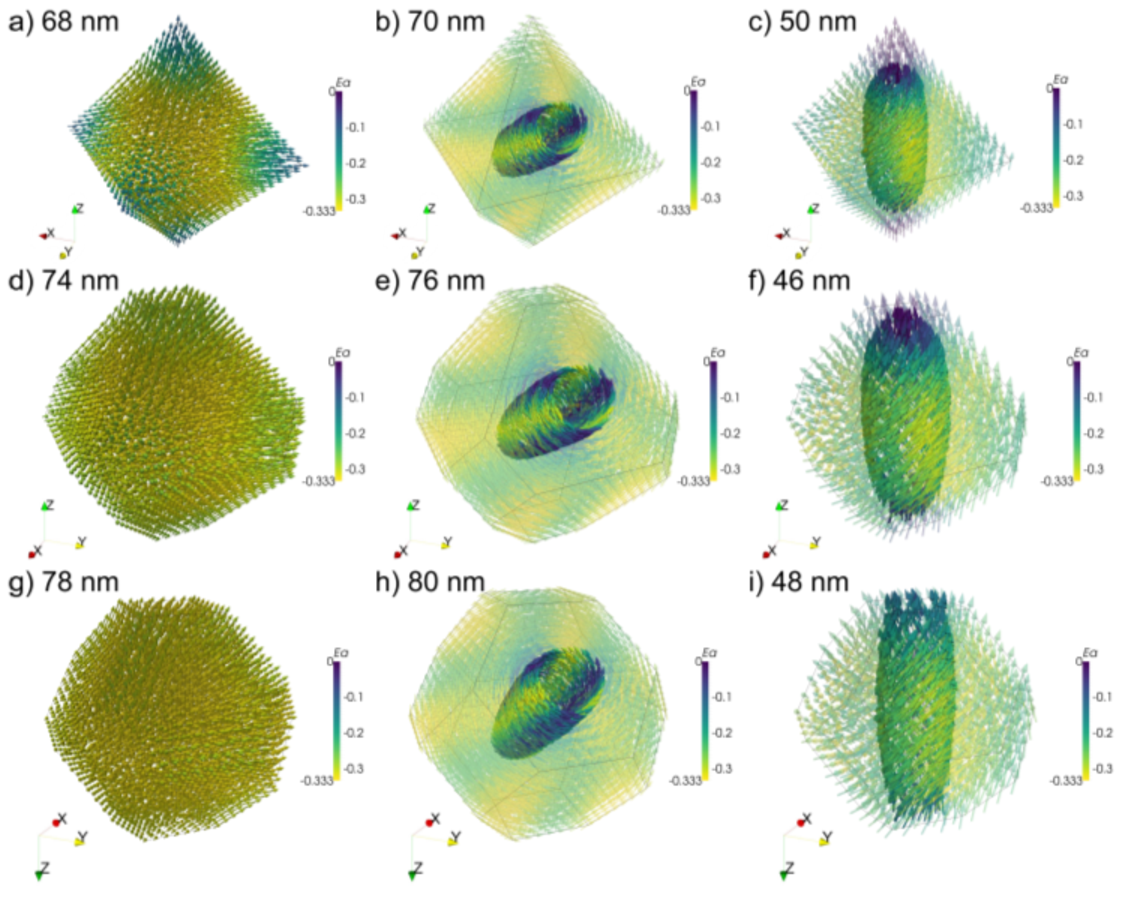
\includegraphics[width=\textwidth]{research-1/figs/Figure_04.pdf}
\caption[Micromagnetic structures of octahedra, minimally truncated octahedra and regular truncated octahedra]{Micromagnetic structures of octahedra, minimally truncated octahedra and regular truncated octahedra. Left column (a, d, g) shows the largest SD solutions at $\dmax$, obtained by interpolating from solutions for smaller grains starting at 30$\nm$. On interpolating to a grain 2$\nm$ larger, the structure relaxes to an EAV (b, e, h), stable up to 120$\nm$. From 120$\nm$ interpolation is carried out into smaller grains. Eventually the vortex aligns with a hard direction (c, f, i) which is stable down to $\dmin$ after which the solution becomes SD again down to 30$\nm$. Top row (a, b, c) shows the structures for the octahedra; center row (d, e, f) for the minimally truncated octahedra and bottom row (g, h, i) for the regular truncated octahedra. Colour represents the MCA energy normalised by $|K_1|$.}
\label{fig4}
\end{figure}

\subsubsection{Cuboctahedra}
The cuboctahedra (Figs. \ref{fig3}i--j) showed a Type 2 ML (Eq. \ref{type2}). The PSD state nucleated on the size-descending curve from the EAV is a distorted IAV (dIAV){\textemdash}a sort of mixed state with the vortex mostly aligned with the [0$\bar{1}$$\bar{1}$] direction and the ends of the vortex deflecting to a hard direction. The ML then has a formula:
\begin{equation}
\text{ML}_{\text{oct.}}^{\text{cub}}=\left(\text{SD}_{30}^{114}\rightarrow\text{EAV}_{116}^{120}\right)_{\rightarrow} + \\
 \left(\text{EAV}_{120}^{86}\rightarrow\text{dIAV}_{84}^{62}\rightarrow\text{HAV}_{60}^{38}\rightarrow\text{SD}_{36}^{30}\right)_{\leftarrow}.
\end{equation}
The SD state is more stable, with $\dmax$ increasing to $\dmax=114\,\text{nm}$ (Fig. \ref{fig5}d) before relaxing to an EAV at 116$\nm$ (Fig. \ref{fig5}e). Growth of the HAV from 60$\nm$ (Fig. \ref{fig5}f) shows a Type A SL (Eq. \ref{typeA}), with the HAV going to the dIAV it nucleated from. The dIAV (Fig. \ref{fig2}f) instead shows a Type B SL. The SL is then:
\begin{equation}
\text{SL}_{\text{oct.}}^{\text{cub}}=\left(\text{HAV}_{60}^{72}\rightarrow\text{dIAV}_{74}^{120}\right)_{\rightarrow} + \left(\text{dIAV}_{84}^{120}\right)_{\rightarrow}.
\end{equation}
\par

\subsubsection{Cubes}
The cubes (Figs. \ref{fig3}k--l) showed a Type 1 ML (Eq. \ref{type1}). The EAV nucleated from the SD state is a distorted EAV (dEAV). The dEAV mostly aligns with an easy direction, but its ends deflect from the vertices to a hard direction, attaching to opposite faces. The ML is then:
\begin{equation}
\text{ML}_{\text{cube}}=\left(\text{SD}_{30}^{80}\rightarrow\text{dEAV}_{82}^{120}\right)_{\rightarrow} + \\
\left(\text{dEAV}_{120}^{64}\rightarrow\text{HAV}_{62}^{38}\rightarrow\text{SD}_{36}^{30}\right)_{\leftarrow}.
\end{equation}
The SD state at $\dmax=80\,\text{nm}$ is largely flowered (Fig. \ref{fig5}g). The dEAV initially nucleated at 82$\nm$ (Fig. \ref{fig5}h) could also be interpreted as a distorted HAV. However, the alignment of such state with an easy direction becomes more obvious for larger cubes. Growth of the HAV from 62$\nm$ (Fig. \ref{fig5}i) results in a Type B SL:
\begin{equation}
\text{SL}_{\text{cube}}=\left(\text{HAV}_{62}^{120}\right)_{\rightarrow}.
\end{equation}
\begin{figure}
\centering
%\includegraphics[width=\textwidth]{Figure_05_HR.pdf}
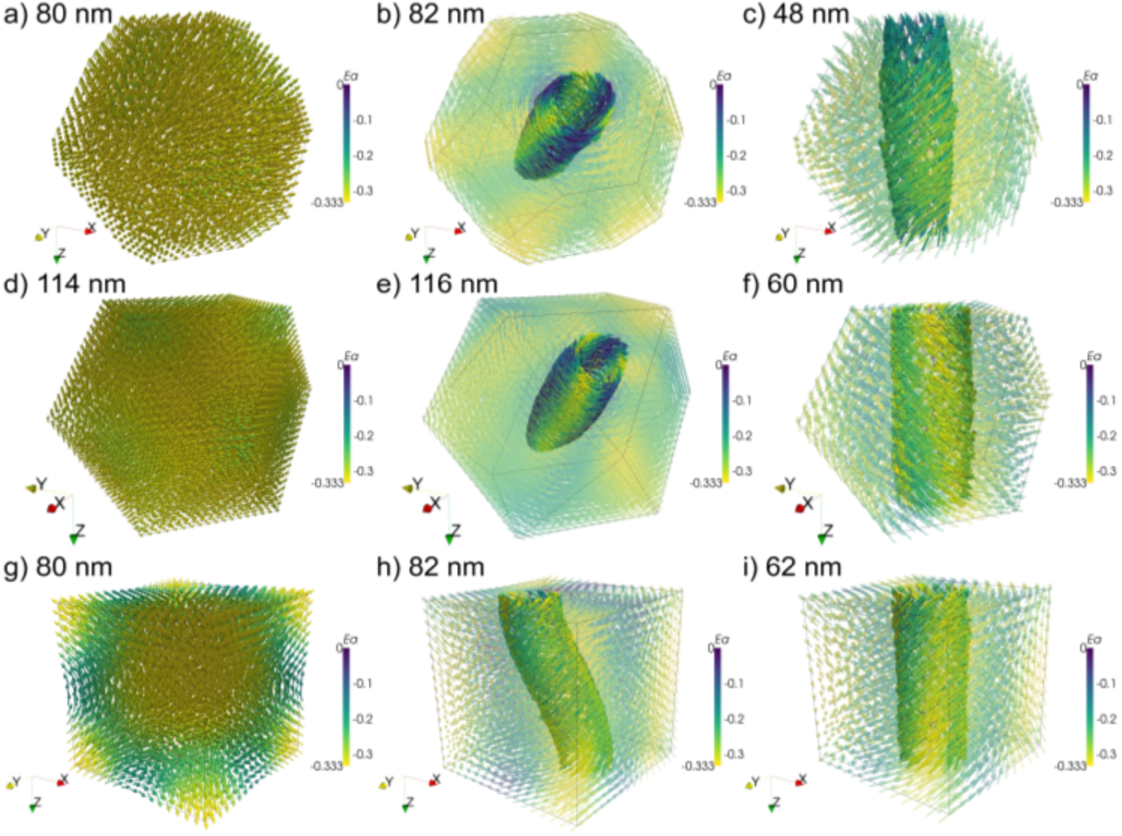
\includegraphics[width=\textwidth]{research-1/figs/Figure_05.pdf}
\caption[Micromagnetic structures of maximally truncated octahedra, cuboctahedra and cubes]{Micromagnetic structures of maximally truncated octahedra, cuboctahedra and cubes. Left column (a, d, g) shows the largest SD solutions at $\dmax$, obtained by interpolating from solutions for smaller grains starting at 30$\nm$. On interpolating to a grain 2$\nm$ larger, the structures relax to an EAV (b, e) or a distorted EAV (h) which are stable up to 120$\nm$. From 120$\nm$ interpolation is carried out into smaller grains. Eventually the vortex aligns with a hard direction (c, f, i), stable down to $\dmin$ after which the solution becomes SD again down to 30$\nm$. Top row (a, b, c) shows the structures for the maximally truncated octahedra; center row (d, e, f) for the cuboctahedra and bottom row (g, h, i) for the cubes. Colour represents the MCA energy normalised by $|K_1|$.}
\label{fig5}
\end{figure}

\subsubsection{Discussion}
The values for $\dmax$ of the spheres are significantly larger than those found for the euhedral shapes (except for the cuboctahedra which have an anomalously large value), perhaps due to the absence of corners to act as nucleation points. Truncation of the octahedral particles increases the (numerical) stability of the SD solutions which is expressed as the increase in $\dmax$ from 68$\nm$ for the octahedra (Fig. \ref{fig3}a) to 114$\nm$ for the cuboctahedra (Fig. \ref{fig3}i) (Table \ref{table1}). A less pronounced effect is the decrease of $\dmin$ with truncation from 46$\nm$ for the octahedra to 38$\nm$ for the cuboctahedra (Table \ref{table1}). HAVs are more (numerically) stable at smaller sizes the more truncated the particle is. This is due to the large stray field energy created by a vortex pointing towards a vertex. It is energetically favourable for a vortex to attach its ends to flat surfaces large enough to accomodate its core. This is seen in the distortion of the vortex structures shown in Figs. \ref{fig2}g, \ref{fig5}h. These avoid the production of large stray fields by attaching their ends to grain faces, at the cost of anisotropy and exchange energies needed to distort the otherwise straight structures of the vortices.\par
\begin{table}[ht]
\centering
\begin{tabular}{| l || c | c | c | c | c | c | c |}
\hline
       & main loop & $\dmax$ & $d_\text{EH}$ & $d_\text{EI}$ & $d_\text{IH}$ & $\dmin$ & $d_0$ \\
\hline
Spheres & T$_1$ & 92 & 54 & N/A & N/A & 40 & 51 \\
\hline
Octahedra & T$_1$ & 68 & 52 & N/A & N/A & 46 & 56 \\
\hline
Min. t. octahedra & T$_2$ & 74 & N/A & 50 & 48 & 44 & 54 \\
\hline
T. octahedra & T$_1$ & 78 & 50 & N/A & N/A & 42 & 53 \\
\hline
Max. t. octahedra & T$_1$ & 80 & 48 & N/A & N/A & 42 & 52 \\
\hline
Cuboctahedra & T$_2$ & 114 & N/A & 86 & 62 & 38 & 50 \\
\hline
Cubes & T$_1$ & 80 & 64 & N/A & N/A & 38 & 52 \\
\hline
\end{tabular}
\caption[Critical sizes for all shapes]{Critical sizes for all shapes. All sizes in nm. $d_0$, $\dmin$ decrease with truncation while $\dmax$ increases.}
\label{table1}
\end{table}

The energy plots (Figs. \ref{fig2}b, \ref{fig3}b, d, f, h, j, l) show the SD energy density is fairly constant with size for all shapes. For the octahedra, the intersection of the EAV and HAV energy curves occurs above the SD curve. This means that it is then the EAV energy curve which first intersects the SD curve at $d_0$ and thus this PSD state becomes the GEM thereon (Fig. \ref{fig3}b). With truncation, this intersection moves closer to the SD curve as can be seen in Fig. \ref{fig3}d in which all the different PSD states (EAV, IAV and HAV) and the SD energy curves meet at roughly the same point. Further truncation causes this intersection to eventually occur below the SD energy curve. This creates a narrow range of sizes for which the HAV is the lowest energy state (Figs. \ref{fig3}f, h). Completely truncated, the cuboctahedra show a \textit{split} of this intersection into distinct crossings of the HAV/IAV and IAV/EAV energy curves (Fig. \ref{fig3}i, compare with Fig. \ref{fig3}d), creating a broad range of sizes, from $\roughly$50$\nm$ to $\roughly$66$\nm$, for which the HAV has the lowest energy. A range for which the HAV has the lowest energy was also found for spheres and cubes. The overall effect of truncation on $d_0$ is to decrease this threshold (Table \ref{table1}).\par

For the cubes we found $\dmax=80\,\text{nm}$, much smaller than the value of 107$\nm$ obtained by \citet{Muxworthy2013}. We found $\dmin=38\,\text{nm}$, in agreement with the value by \citet{Muxworthy2013}. We found the intersection of the SD and HAV energy curves $d_0\approx 52\,\text{nm}$ (Fig. \ref{fig3}l), lower than the value of 58$\nm$ by \citet{Muxworthy2013}. Modelling the ML for cubes with the $M_\text{S}$ value used by \citet{Muxworthy2013} we obtained $\dmax=92\,\text{nm}$, $\dmin=42\,\text{nm}$ smaller and larger, respectively, than the values by \citet{Muxworthy2013}. The differences in $\dmax$, $\dmin$ can be due to \citet{Muxworthy2013} using a FD method as opposed to a FEM used here. However, excellent agreement of $d_0\approx 60\,\text{nm}$ was found with the value of 58$\nm$ by \citet{Muxworthy2013}. The difference between $d_0$ obtained with the different $M_\text{S}$ is significant as it is larger than the exchange length and thus, unlikely to be an effect of discretisation.\par

\subsection{Identifying the PSD--MD transition}
Unlike fine SD grains, bulk ferromagnetic materials can possess a (roughly) null net magnetisation. This is because bulk ferromagnets, in their lowest energy state, have a multi-domain (MD) magnetic structure \citep{Dunlop}. MD structure is characterised by the coexistence of multiple magnetic domains: small regions saturated in different easy directions and separated by narrow planar regions called domain walls where the magnetisation vector transforms continuously from the direction of one domain to that of its neighbour. Near the surface of a bulk sample the magnetic domains lie in directions parallel to the surfaces, which do not necessarily coincide with the magnetocrystalline easy axes; these are called \textit{closure domains} as they enclose the magnetic flux. Then, MD grains minimise the stray field energy at the expense of exchange and MCA energies associated with the domain walls and closure domains. This balance becomes more energetically favourable as a particle grows. To identify a plausible PSD--MD transition, EAV states found to be stable at 120$\nm$ were further grown up to 300$\nm$ in steps of 2$\nm$.\par

\subsubsection{Growth of EAVs}
The octahedron EAV (Fig. \ref{fig4}b) was found to remain stable up to 300$\nm${\textemdash}as was the case for the EAVs for all shapes. However, although the overall structure is preserved as the grain grows, there is a gradual, continuous transformation towards MD structure. As the crystal becomes larger, the vortex core (the cylindrical region encompassing the highest helicity $K=\boldsymbol{m}\cdot\nabla\times\boldsymbol{m}$) width remains the same. The regions radially far from the core become screened from its influence and more influenced by the effects of MCA, giving way to six ever larger expanses of the grain that become magnetised along easy axes. The sections with higher MCA energy become increasingly narrower, more planar and confined between the easy-aligned regions. With further growth, the regions close to the edges become magnetised along the edges thus completing a picture of MD structure: magnetic domains magnetised along easy directions (Fig. \ref{fig6}a); flat, narrow magnetic domain walls dividing these and closure domains formed along edges of the body (Fig. \ref{fig6}b). The spheres (not shown) show this same general behaviour of formation of magnetic domains and domain walls, but without the formation of closure domains as there are no edges to nucleate these type of domains.\par

At 300$\nm$, the regular truncated octahedron shows the same basic structure as the 300$\nm$ octahedron except for the widening of the domain walls as they approach the square $\{$001$\}$ faces (Figs. \ref{fig6}c--d). Completely truncated, the cuboctahedra have a somewhat different structure. In the 300$\nm$ cuboctahedron solution the domain walls have become so wide as they draw closer to the square faces that they engulf three of the magnetic domains (Fig. \ref{fig6}e), and hard-aligned N\'eel walls appear which are visible as blue streaks on the square faces (Fig. \ref{fig6}f).
\begin{figure}
\centering
%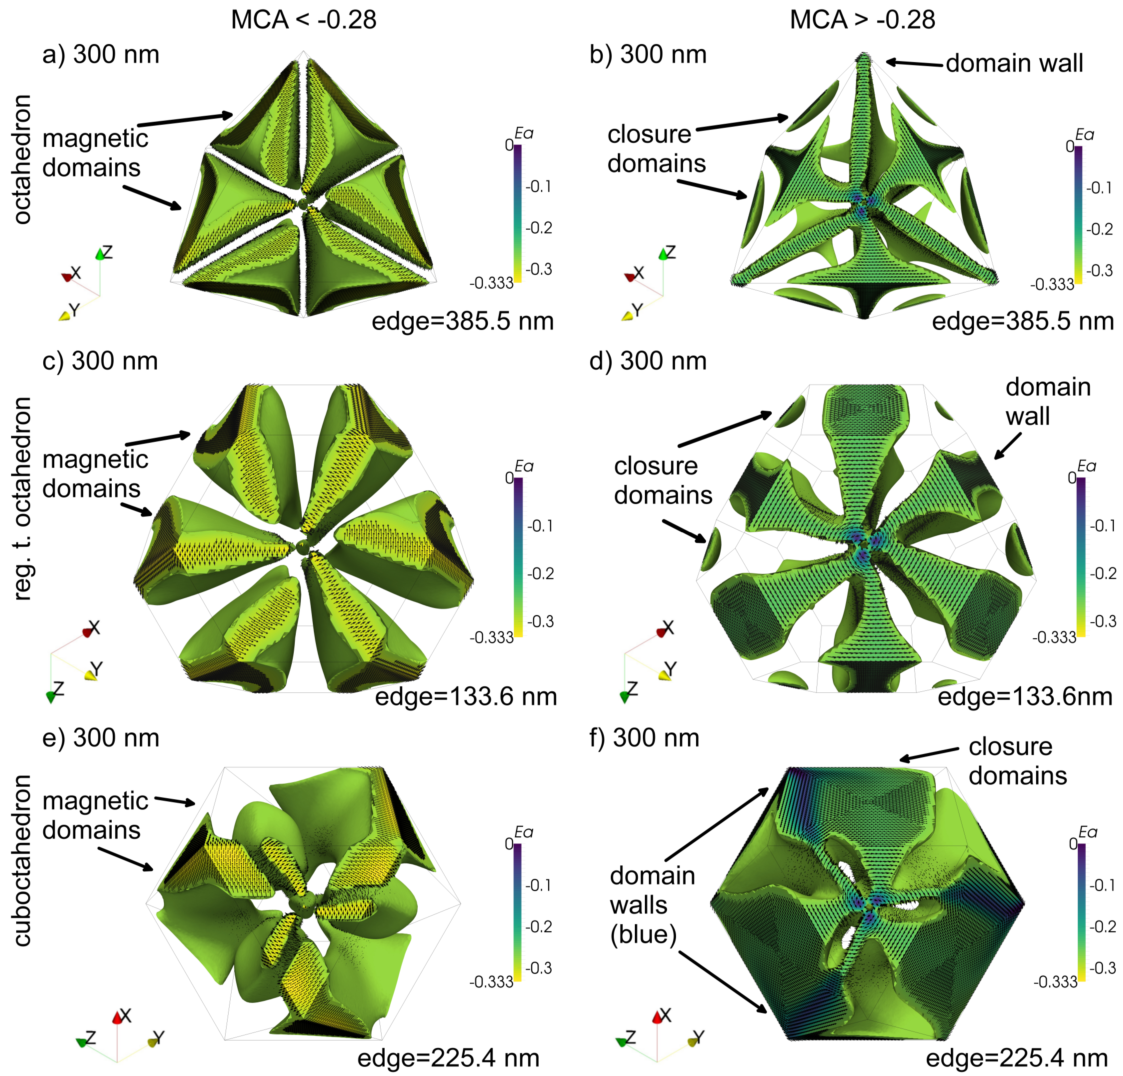
\includegraphics[width=\textwidth]{Figure_06_HR.pdf}
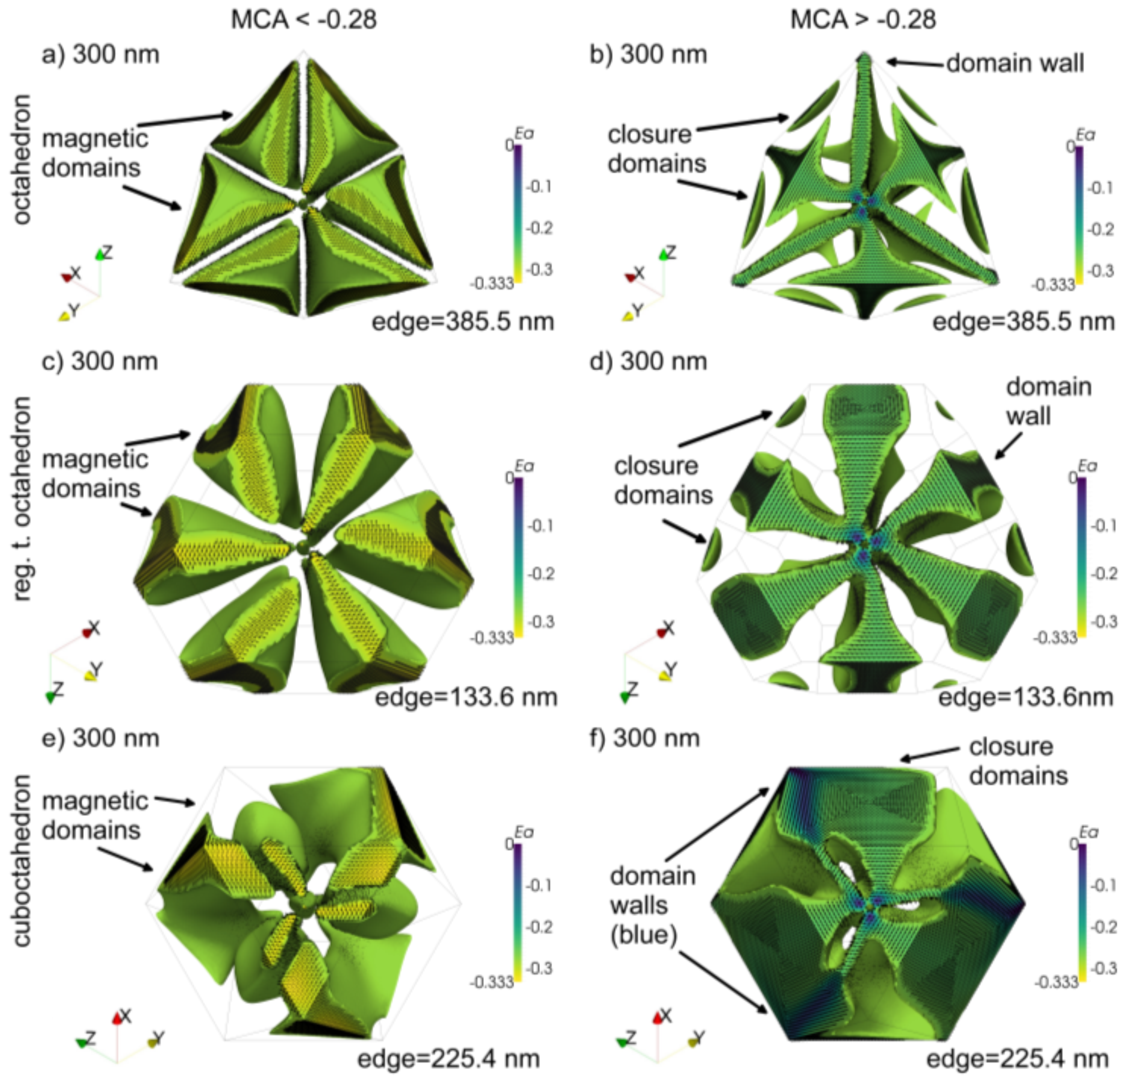
\includegraphics[width=\textwidth]{research-1/figs/Figure_06.pdf}
\caption[MD formation by easy aligned vortices]{MD formation by easy aligned vortices. From the solutions obtained by growing the 120$\nm$ EAVs up to 300$\nm$, the mesh nodes with MCA energy $<$-0.28 (normalised by $|K_1|$) are shown in the left column (a, c, e). These are regions which deviate from an easy axis alignment by less than $\roughly$15$^{\circ}$. The complement is shown in the right column: the regions with moderate to high ($>$-0.28) MCA energy (b, d, f). In the octahedron, there form six large magnetic domains filling up most of the volume (a) and narrow, flat regions acting as domain walls and small wedge-like regions formed along the edges interpreted as closure domains (b). The regular truncated octahedron EAV grown up to 300$\nm$ shows the same pattern: large magnetic domains with low MCA energy occupy most of the volume (c); the effect of truncation (and consequent creation of $\{001\}$ surfaces) is to widen the domain walls as they approach the surfaces as this reduces the stray field energy (d). Closure domains along the edges are still pronounced (d). Fully truncated, the effect on the structure of the cuboctahedron EAV grown to 300$\nm$ is to reduce the proportion of the volume occupied by magnetic domains (e). The domain walls are so wide close to the surfaces that they engulf three of the domains, while also hard-aligned N\'eel walls are formed as seen from the blue streaks on the surface (f). Colour represents the MCA energy normalised by $|K_1|$.}
\label{fig6}
\end{figure}

\subsubsection{Discussion}
A tentative mechanism for a PSD--MD transition has been identified. This proceeds by a gradual formation of magnetic domains, domain walls and closure domains `seeded' by the vortex structures nucleated in the SD--PSD transition regime. However, this transition is more obvious for the octahedra than the truncated octahedra and cuboctahedra.\par

Since our models do not account for the effects of thermal fluctuations, the stability of the solutions is only numerical, e.g., the energy landscape of a micromagnetic solution is somewhat flat in the vicinity of the solution, thus small numerical perturbations can be insufficient for a micromagnetic algorithm to drive the solution to a new local energy/torque minimum depending on the sensitivity or control parameters of the algorithm. We find for the octahedra and the cuboctahedra two solutions for each morphology up to 300$\nm$ (Figs. \ref{fig3}a, e). Although the EAVs for both have the lowest energies, this leaves open the question of whether we can expect to find metastable grains with the higher energy structures. Likewise, in Section \ref{sd-psd} we find that grains remain SD beyond $d_0$. In theory, a particle can remain in a metastable SD state beyond this threshold if the energy barrier separating the SD from the PSD state is higher than the thermal energy available. Knowledge of the energy barriers near the SD--PSD transition is needed to answer these questions.\par

\subsection{Energy barriers and blocking volumes}
A nudged elastic-band (NEB) method \citep{Fabian2017} was implemented for the calculation of the energy barriers at room temperature as a function of size and shape for the (truncated) octahedral morphologies. To calculate the energy barrier for a given shape and size we obtain many solutions from randomised initial conditions. From this set of solutions the state with the lowest energy is identified. For the smaller particles we expect the GEM to be SD and for larger grains PSD. Once the GEM has been identified from the set of initial solutions, two appropriate solutions must be chosen to calculate the action-minimising path (AMP) between them and thus the energy barrier.\par

When the GEM is a $<$111$>$-aligned SD state, the pair of appropriate solutions are magnetised normal to contiguous $\{$111$\}$ faces. Above $d_0$ the GEM is usually a HAV, then, the paths to test are between vortices at 90$^{\circ}$ from each other, e.g., between [100] and [001] vortices. For some shapes the GEM is a distorted vortex, for these, it is important to calculate several paths between different configurations to find the transition with the lowest energy barrier. At larger sizes, for all shapes the GEM is an EAV, this means that the paths to calculate are between vortices pointing towards contiguous $\{$111$\}$ faces, much like for SD particles. For all PSD to PSD transitions the vortices must have the same chirality as a change produces prohibitively large energy barriers one to two orders of magnitude larger than the AMP barrier and thus we can neglect the possibility of such transitions. It is not necessary to calculate the energy barriers for transitions other than the ones with the lowest energy as these dominate the behaviour and higher energy transitions usually proceed via lower energy ones \citep{Nagy2017}. For perfectly regular, equant grains as those modelled in this study, the lowest energy transition is degenerate and so, the relaxation time has to be divided by three (for the three distinct degenerate paths).\par

\subsubsection{Octahedra and truncated octahedra}
Fig. \ref{fig7} shows three examples of transitions for the regular truncated octahedra which were found to be typical for all the (truncated) octahedra, but for the cuboctahedra. At the smaller sizes (Fig. \ref{fig7}, left column) the transition is from SD to SD via coherent rotation. The energy along such a path is plotted in Fig. \ref{fig7}a; the energy barrier is the difference between the easy (Figs. \ref{fig7}d, j) and intermediate-aligned SD (Fig. \ref{fig7}g) energies. The energy barrier for such transitions, for all shapes, is quite low, with relaxation times from a few microseconds to a few days for the largest of these. A few nanometers before the SD--PSD transition the AMP is not a coherent rotation, but a transition via a curling mode (Fig. \ref{fig7}, center column). The energy barrier is also the difference between the easy and intermediate-aligned SD energies.\par

Once the GEM is an EAV, the transitions are between isochiral EAVs directed towards contiguous $\{$111$\}$ faces (Fig. \ref{fig7}, right column). The transition is a structured rotation of the vortex, through an IAV (Fig. \ref{fig7}i), which maintains its overall shape along the path. The energy along such paths is a double-bump where the IAV sits in a shallow local energy minimum (LEM). This means that the energy barrier is not the difference between the EAV and IAV energies. Rather, it is given by the barrier separating the EAV from the IAV. However, with increasing size the IAV LEM becomes more shallow and thus the energy barrier is better approximated by the difference between the EAV and IAV energies{\textemdash}at 64$\nm$ the IAV LEM is so shallow that the double-bump feature becomes flattened (Fig. \ref{fig7}c). In general, the PSD to PSD transitions are very similar to coherent rotations between SD states in that they are structured rotations of the vortex core. The left column of Video 1 (supplementary material) shows these typical transitions.
\begin{figure}
\centering
%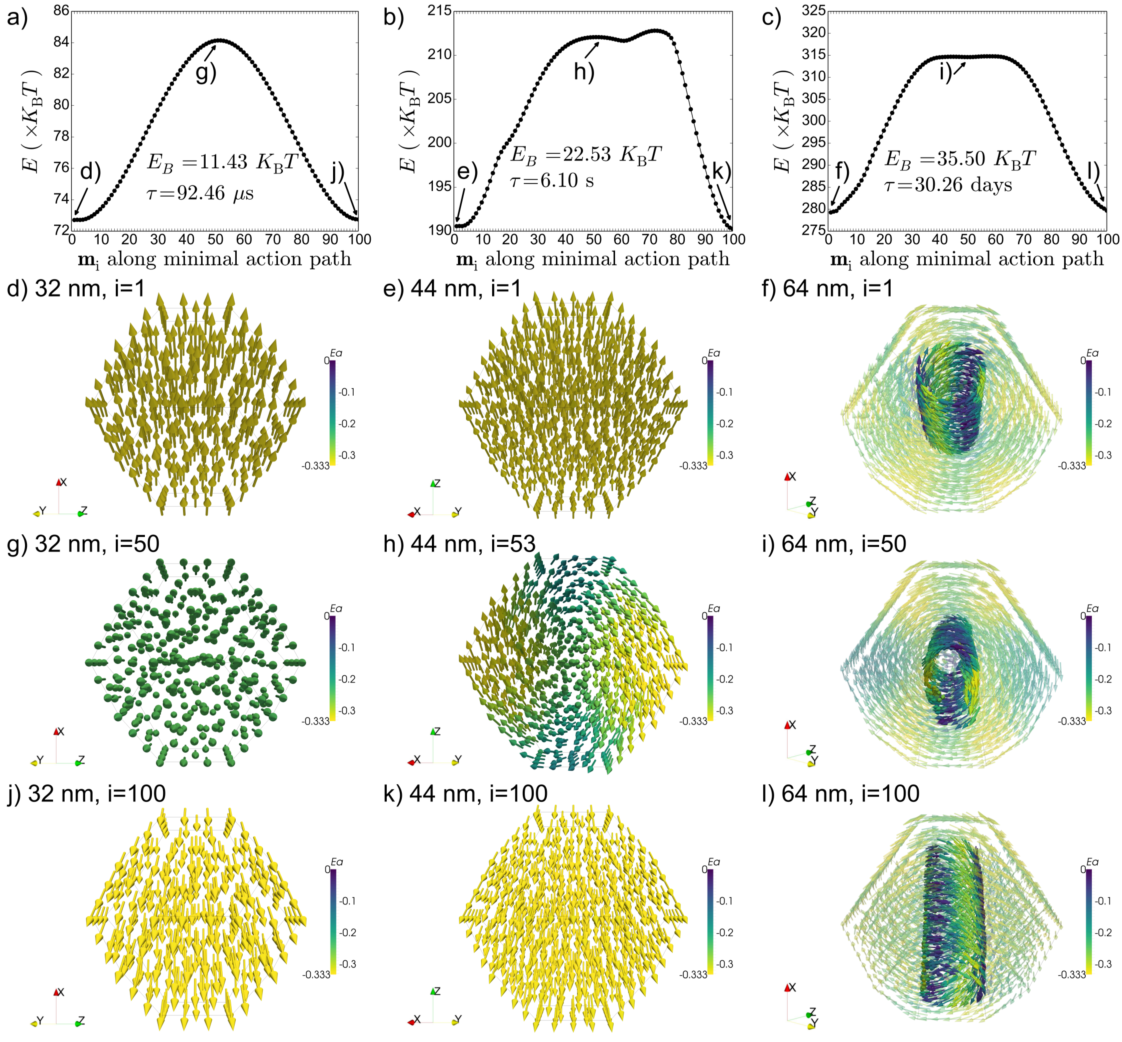
\includegraphics[width=\textwidth]{Figure_07_HR.pdf}
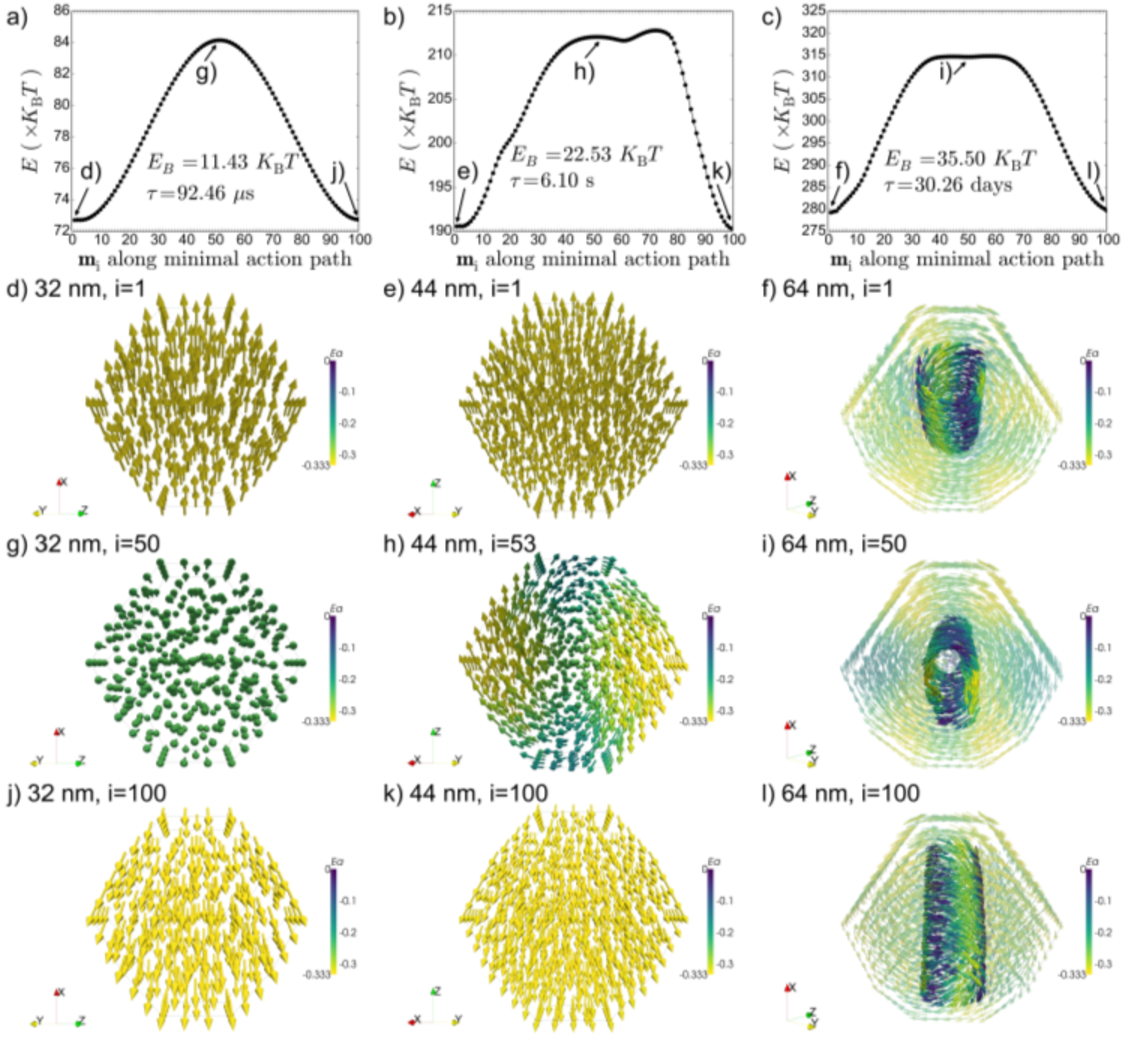
\includegraphics[width=\textwidth]{research-1/figs/Figure_07.pdf}
\caption[Typical action-minimising paths]{Typical action-minimising paths. The regular truncated octahedra illustrate the typical AMPs found for all the (truncated) octahedral shapes. Well below the SD--PSD threshold the AMP between SD configurations is a coherent rotation (left column). The energy along the AMP is a single bump (a) and the energy barrier is an intermediate-aligned SD state (d). At sizes just below the SD--PSD threshold the AMP is still between SD states, but via a curling mode (vortex nucleation) (center column). Starting from SD (e), a vortex is nucleated (h) then unwinds to an intermediate-aligned SD state which has the highest energy along the AMP (not shown). Then, the final SD state (k) is reached via coherent rotation. This makes the energy along the AMP more complex and asymmetric (b). Well above the SD--PSD threshold, once the EAV has the lowest energy, the AMP is via a structured rotation of the vortex core (right column). The transition is between two EAVs with the same chirality (f, l) as a change of chirality produces prohibitively large energy barriers. In the AMP there is an IAV sitting in its own shallow LEM (i). The energy barrier is the one that separates the EAVs from the IAV. However, as the grain grows, the IAV LEM becomes more shallow and the energy along the AMP flattens (c). Colour represents the MCA energy normalised by $|K_1|$. The energies along the AMPs are plotted in units of $K_\text{B}T$, with $T=300\,\text{K}$. The left column of Video 1 (supplementary material) shows these transitions.}
\label{fig7}
\end{figure}

\subsubsection{Cuboctahedra}
The cuboctahedra show a very different behaviour. Their relaxation times increase exponentially for the SD to SD transitions, but do not drop for the first PSD to PSD transitions, at 48$\nm$, which are hard-aligned to hard-aligned (Fig. \ref{fig8}, left column) and pass through a dIAV (Fig. \ref{fig8}g). The energy barrier is an IAV (Fig. \ref{fig8}j). The relaxation times for these transitions then decrease as the HAV and dIAV energies get closer until, at 66$\nm$, the GEM is a dIAV. Then, since the straight IAV has a very high energy, transitions in which the dIAV ends reattach to contiguous faces are unfavorable. The transition with the lowest energy barrier is between two distorted vortices like the ones shown in Figs. \ref{fig8}e, k, which are (though distorted) [0$\bar{1}\bar{1}$]- and [1$\bar{1}$0]-aligned. The transition preserves the shape of the distorted vortex as it structuredly rotates keeping its ends attached to the square faces.\par

The relaxation times for this type of transitions plateau at a few microseconds up to 74$\nm$. In Fig. \ref{fig3}j the energies of the dIAV and the EAV intersect at roughly 90$\nm$ and are very close up to 120$\nm$. Since the transition between two EAVs is likely to go through a dIAV, it is not expected that the relaxation time for EAV to EAV transitions will rapidly increase until sizes much larger than 90$\nm$. Indeed, we find that only for the particles larger than 110$\,$nm the relaxation times start to grow exponentially{\textemdash}though at a rate slower than for (truncated) octahedra transitions{\textemdash}surpassing 4 billion years at roughly 134$\nm$ (Fig. \ref{fig9}c). A typical transition of this type at 132$\nm$ is shown on the right column of Fig. \ref{fig8} between [111]- and [11$\bar{1}$]-aligned vortices via vortex distortion (not shown). The highest energy state along the path is a straight IAV (Fig. \ref{fig8}i). The right column of Video 1 (supplementary material) shows these transitions.
\begin{figure}
\centering
%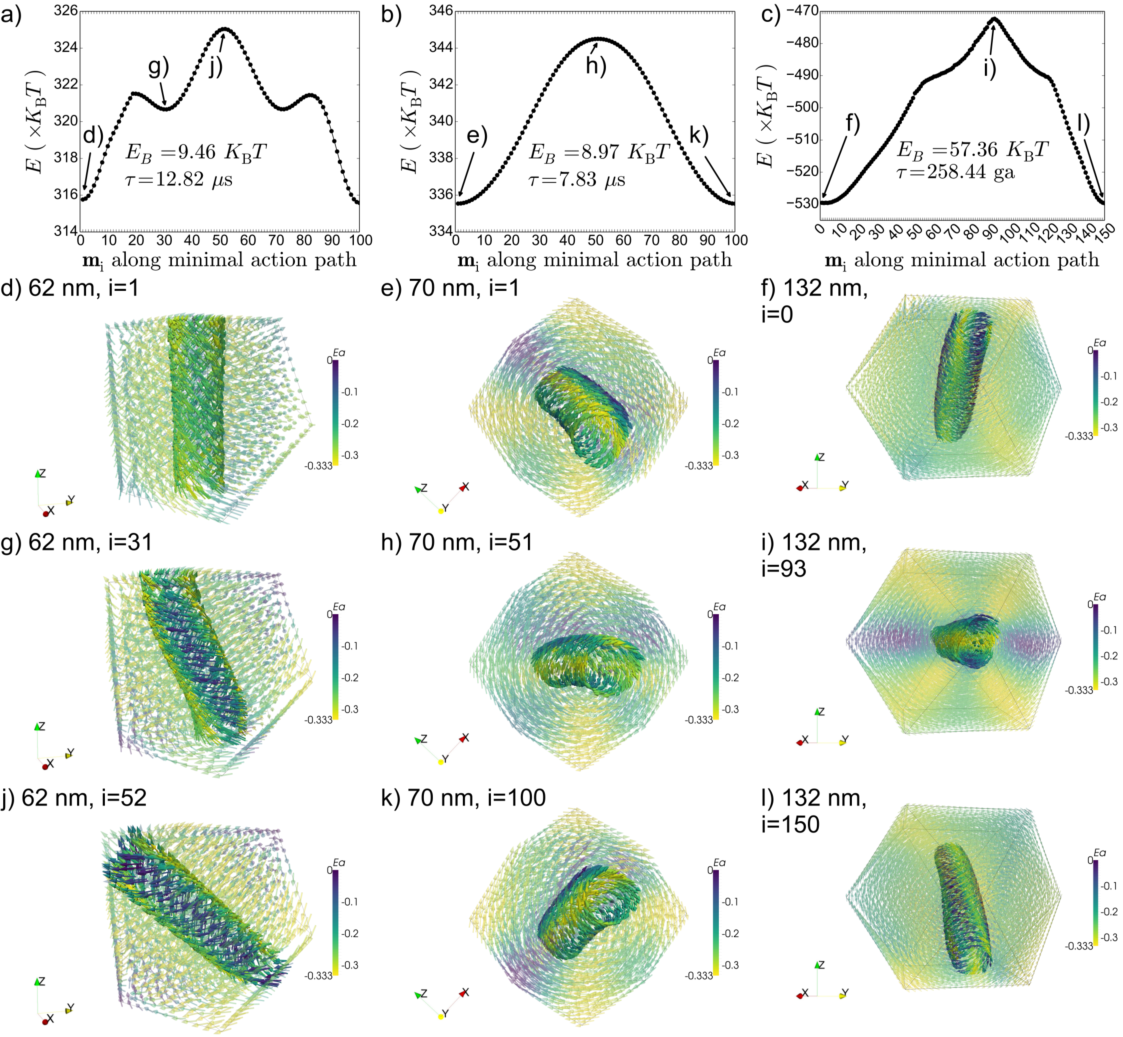
\includegraphics[width=\textwidth]{Figure_08_HR.pdf}
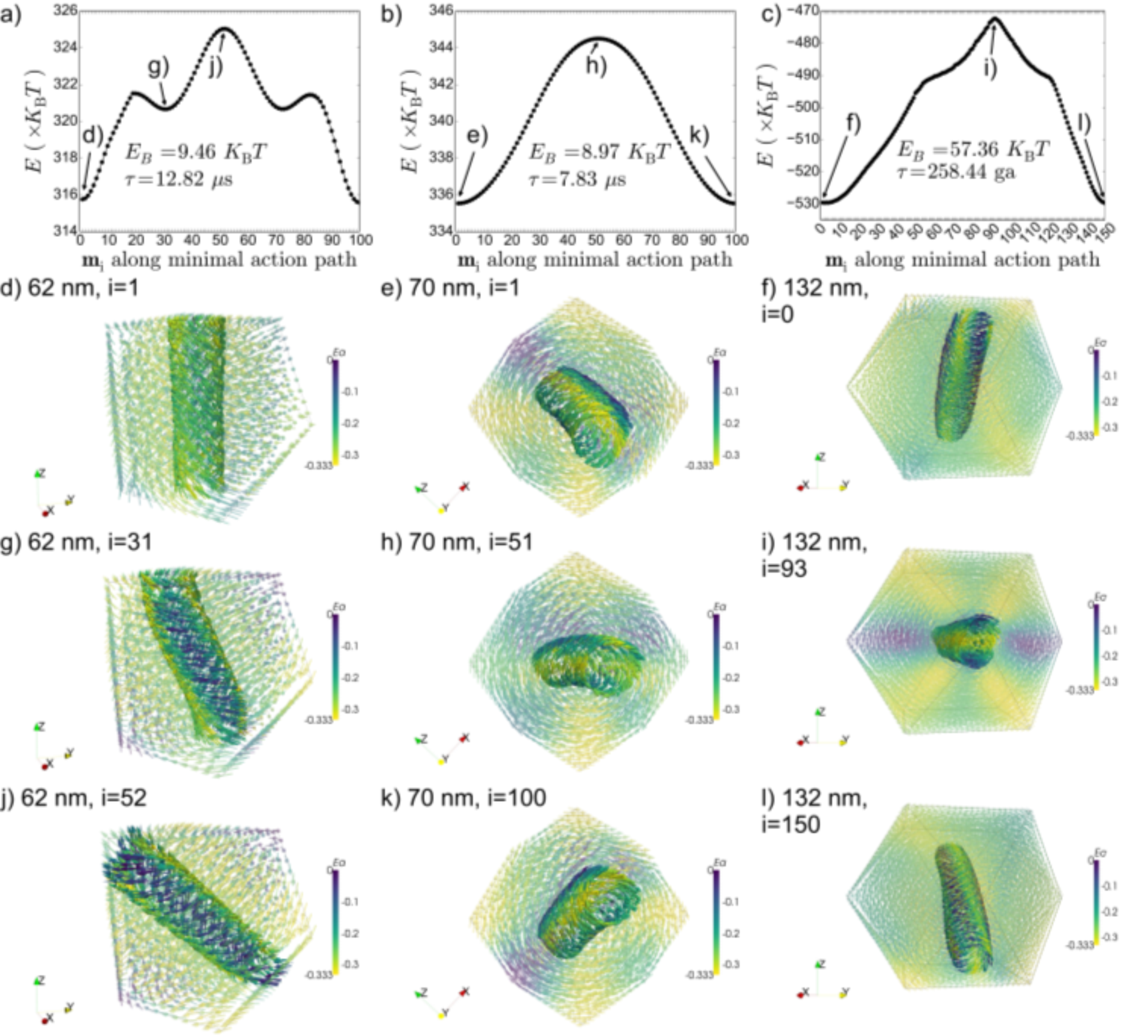
\includegraphics[width=\textwidth]{research-1/figs/Figure_08.pdf}
\caption[Action-minimising paths for the cuboctahedra]{Action-minimising paths for the cuboctahedra. The cuboctahedra showed different AMPs above the SD--PSD threshold from the rest of the shapes. Above the SD--PSD threshold, and up to 66$\nm$, the lowest energy state for the cuboctahedron is a HAV. Transitions between HAVs (left column) occur via a distortion (g) and structured rotation (j) of the vortex core. The energy barrier is an IAV (j). The dIAV along the AMP (g) sits in its own LEM, forming a three-bump energy barrier (a). The dIAV becomes the lowest energy from 66$\nm$. Transitions between dIAVs (center column) form a single bump energy barrier (b). The transition is a structured rotation of the distorted vortex, keeping attached to the same surface (e, h, k). Once the lowest energy is an EAV, transitions between these (right column) occur via a distortion and structured rotation of the vortex core. The energy barrier is an IAV (i). Colour represents the MCA energy normalised by $|K_1|$. The energies along the AMPs are plotted in units of $K_\text{B}T$, with $T=300\,\text{K}$. The right column of Video 1 (supplementary material) shows these transitions.}
\label{fig8}
\end{figure}

\subsubsection{Discussion}
Fig. \ref{fig9} summarizes the results of the relaxation times obtained for the five (truncated) octahedral shapes in the 30$\nm$ to 74$\nm$ range and the relaxation times for the cuboctahedra in the 120$\nm$ to 134$\nm$ range (Fig. \ref{fig9}, inset). For all shapes, except the cuboctahedral, the general behaviour is an exponential increase of the relaxation times for the SD to SD transitions from a few tens of microseconds to a few seconds for the regular truncated octahedra and up to 12 days for the octahedra, followed by a sharp drop at 46$\nm$ (for the regular truncated octahedra) to 50$\nm$ (for the octahedra). This drop in the relaxation times marks the SD--PSD threshold. Then, the PSD to PSD transitions have increasingly lower relaxation times until reaching a global minimum at $\roughly$50$\nm$ to $\roughly$54$\nm$. Once the GEM is the EAV the relaxation time shoots up exponentially with crystal growth, surpassing 4 billion years at $\roughly$68$\nm$ to $\roughly$72$\nm$.
\begin{figure}
\centering
%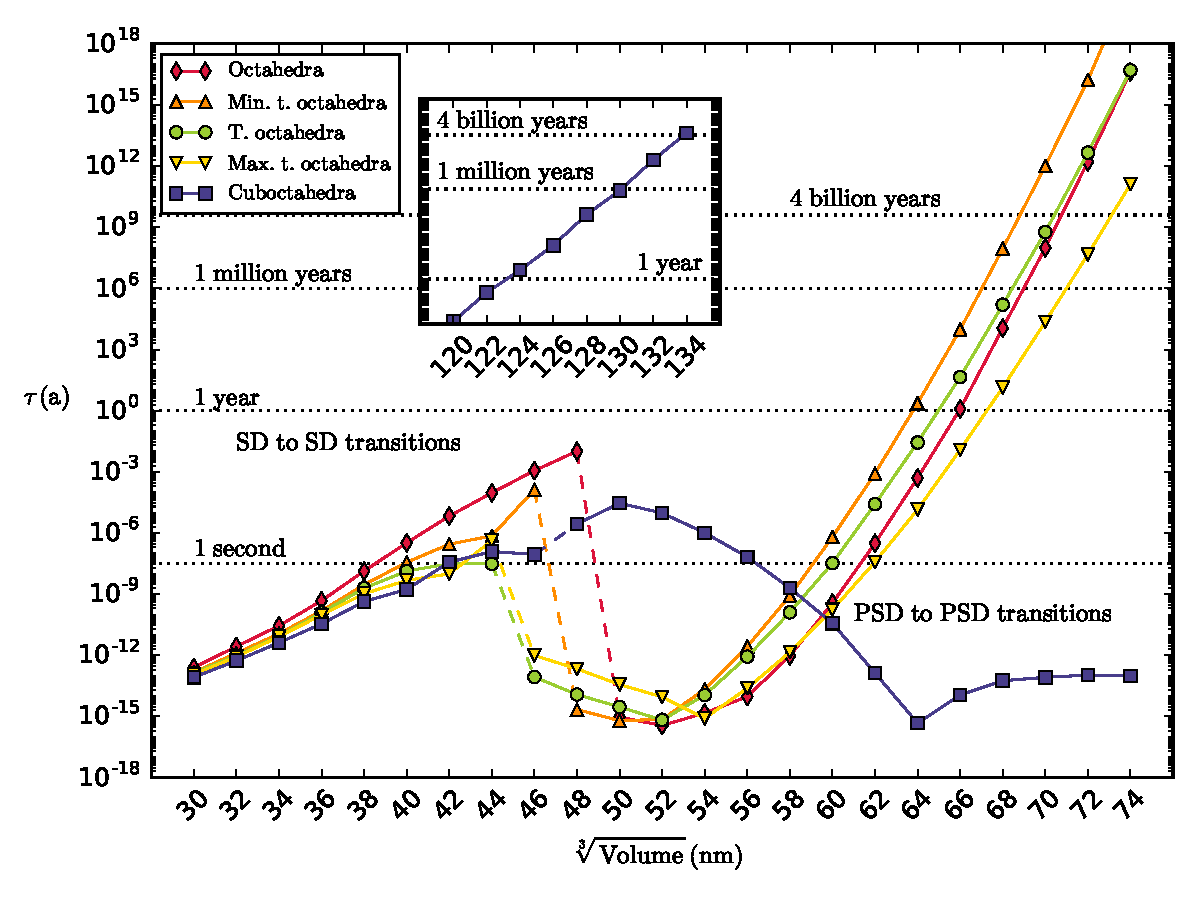
\includegraphics[width=\textwidth]{Figure_09_HR.pdf}
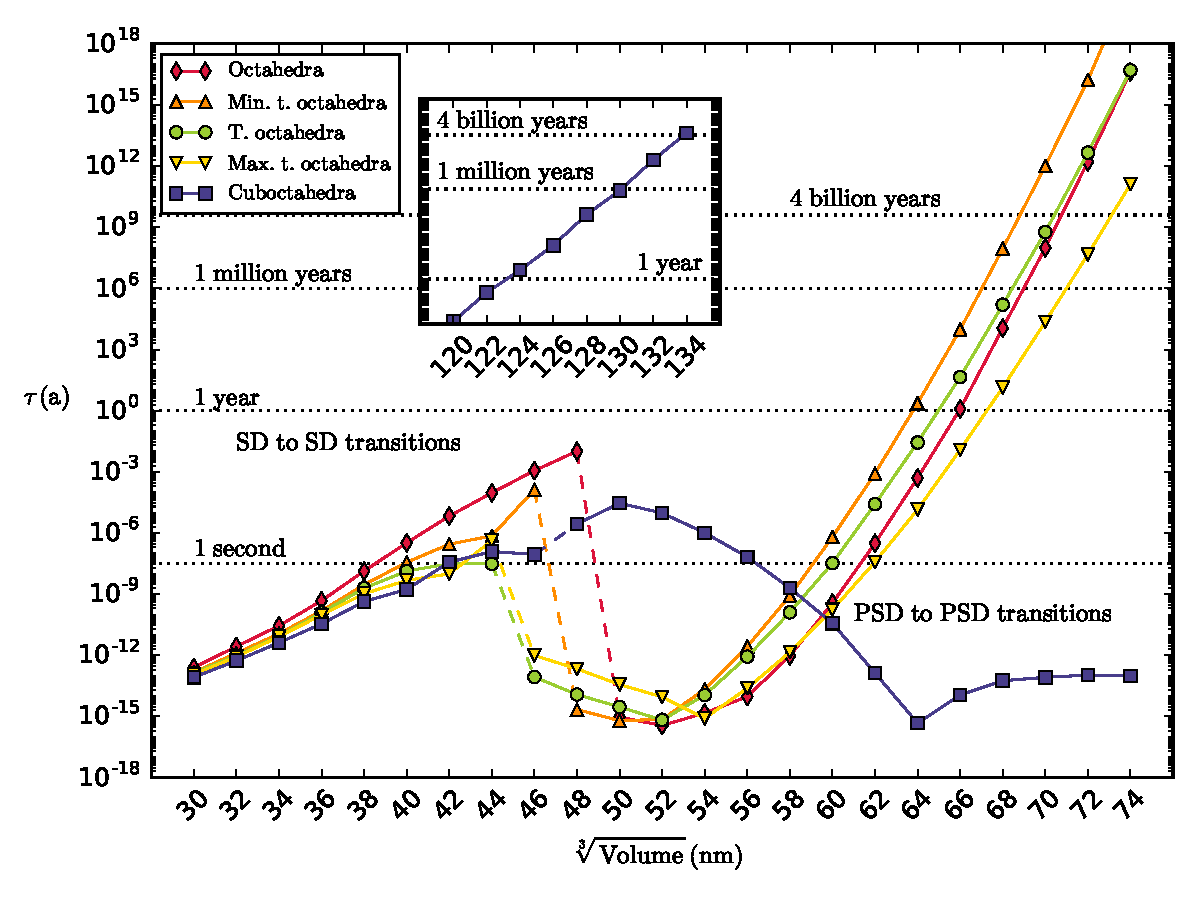
\includegraphics[width=\textwidth]{research-1/figs/Figure_09.pdf}
\caption[Relaxation times for the euhedral shapes]{Relaxation times for the euhedral shapes. The relaxation times are calculated with $\tau_0=1\,\text{ns}$, $T=300\,\text{K}$. $\tau$ increases exponentially for the SD--SD transitions, but reaches only laboratory scale stabilities before the SD--PSD threshold. The (truncated) octahedral shapes show a dip in the stability in the lower end of the PSD range for HAV--HAV and IAV--IAV transitions, reaching a minimum at $\roughly$52$\nm$. Once the EAVs have the lowest energies, the relaxation times grow exponentially with size, reaching four billion years from $\roughly$70$\nm$. The cuboctahedra, however, show a different behaviour: they do not show a dip in the stability for the first HAV--HAV transitions, but with increasing size they produce lower relaxation times as the energy of the dIAV gets closer. The relaxation times for the transitions between dIAVs plateau up to 74$\nm$. Exponential growth of the relaxation times occurs from $\roughly$110$\nm$ (inset), surpassing four billion years from $\roughly$134$\nm$.}
\label{fig9}
\end{figure}

These calculations show that equant, non-interacting, room-temperature SD grains of greigite are on a geological timescale, SP given that the largest relaxation time found for SD particles (octahedra) of 12 days is only stable on laboratory timescales. Therefore, the expected SP--SSD threshold does not exist but rather a SP--PSD threshold since it is only the PSD grains which can hold a remanence for extended periods of time. \citet{Muxworthy2013} estimated the energy barriers for non-interacting cubes of greigite from the anisotropy energy surface and found a SP--SSD threshold of 56$\nm$, for a relaxation time of four billion years. In this study the blocking volumes for cubes and spheres were not calculated as these are not naturally occurring morphologies for greigite. However, given the results for the five (truncated) octahedral shapes, it is unlikely that a SP--SSD threshold should exist for either cubes or spheres.\par

Since the relaxation times for the larger SD particles are so small and since the transitions from SD to SD just before the GEM becomes PSD are through a curling mode (vortex nucleation), we conclude that the SD--PSD threshold is defined only by the first intersection of a PSD energy curve with the SD energy curve, $d_0$ (Figs. \ref{fig2}b, \ref{fig3}b, d, f, h, j, l). That SD--SD transitions just below the SD--PSD threshold occur via a curling mode was also observed for magnetite by \citet{Enkin1994} and shows that greigite particles are likely to show PSD aspects even below the SD--PSD threshold. It is highly unlikely that metastable SD grains exist beyond $d_0$ in the absence of grain--grain interactions. The relaxation times between PSD states just above $d_0$ are the shortest of all and only start to grow exponentially for the EAV to EAV transitions. We thus conclude that the PSD--MD transition through a crystal growth mechanism, must occur through an EAV path.\par

The splitting of the energy curves' intersections exhibited by the cuboctahedra not only has repercusions on the SD--PSD threshold, but also on its stability against thermal fluctuations. All the (truncated) octahedral particles have blocking volumes of $\roughly$72$\nm$ while for the cuboctahedra this volume is $\roughly$134$\nm$. This could be explained by the fact that the first PSD to PSD transitions, between hard-aligned PSD states, traverse through IAVs (Fig. \ref{fig8}, left column): as the cuboctahedral particle grows, the energy difference between the IAV and HAV becomes smaller (Fig. \ref{fig3}j) and this is reflected in a diminishing of the relaxation times for this type of transition (Fig. \ref{fig9}). Since for the rest of the shapes the PSD and SD energy curves all meet in a relatively short span, this effect of diminished stability with increasing size only lasts for a much smaller range of sizes, and once the EAV is the GEM, the relaxation times for transitions between this type of domain state grow very rapidly. However, for the cuboctahedra the EAV becomes the GEM at a larger size than for the rest of the shapes and the energy difference with the dIAV, through which the AMP goes through, is very small.\par
%-----------------------------------------------------

\section{Conclusion}
We have presented calculations of the SD--PSD threshold for realistic shapes of equant greigite grains. We have found that octahedral shapes have the largest SD--PSD threshold $d_0\approx56\,\text{nm}$, a value lower than the threshold obtained for magnetite octahedra by \citet{Witt2005} of $\roughly$73$\nm$. This value decreases by the effects of truncation to $d_0\approx53\,\text{nm}$ for the regular truncated octahedra and further down to $d_0\approx50\,\text{nm}$ for the cuboctahedra. The SD--PSD threshold for greigite cubes was lower ($d_0\approx 52\,\text{nm}$) than that of \citet{Muxworthy2013} (=58$\nm$); however, we used a different value for $M_\text{S}$. When we modelled using the same parameters as \citet{Muxworthy2013} we found excellent agreement, obtaining a $d_0\approx 60\,\text{nm}$.\par
NEB method calculations of the room-temperature blocking volumes of greigite show the importance of thermal fluctuations in determining the magnetic structure of a ferromagnetic grain beyond simpler micromagnetic models. We found that equant SD greigite grains cannot be expected to be reliable palaeomagnetic recorders: only PSD grains larger than $\roughly$72$\nm$ are able to hold a remanence in geological timescales, though there is a strong grain shape dependence.\par

We found that cuboctahedral particles have a blocking volume of $\roughly$134$\nm$, a volume almost seven times larger than for the (truncated) octahedral particles. This highlights the importance of addressing not only the size distribution in sedimentary rock samples, but also the shapes of the greigite grains present.\par
We found that the transitions between PSD states occur via well-defined states by a structured rotation of the vortex cores. This could be useful for future analytical models beyond the SD coherent rotation theory.\par

Although in this study we have disregarded the effects of particle elongations, which are sure to effect the blocking volumes \citep{Muxworthy2013}, our results are representative of widespread authigenic greigite grains of abiotic origin. The effects of grain--grain magnetostatic interactions have also been excluded from this study. Isolated greigite grains are not very common, rather, natural samples show that greigite is more commonly aggregated in tight clusters. However, this study provides a stepping-stone towards understanding the more complex greigite clusters.\par

%-----------------------------------------------------
\renewcommand\bibname{{References}}
\bibliographystyle{elsarticle-harv}
\bibliography{references}
%-----------------------------------------------------
